% =====================================================================
% Chapter 3: Methodology
% =====================================================================
\chapter{Methodology}
\label{ch:methodology}

\section{Overview}

This chapter describes the datasets, pre-processing techniques, model
architectures, and evaluation metrics used across the two pipelines
developed for this thesis. The \textbf{image-based pipeline} is
implemented in the notebook \mbox{\texttt{jersey\_recognition\_images.ipynb}},
and the \textbf{video-based pipeline} is implemented in
\mbox{\texttt{jersey\_recognition\_videos.ipynb}}. Both were executed on
Kaggle cloud GPU runtimes.

\section{Datasets}
\label{sec:datasets}

\subsection{SoccerNet SN-Jersey (Image Pipeline)}

The image pipeline uses the \textbf{SoccerNet SN-Jersey-2023} dataset,
downloaded using the \texttt{SoccerNetDownloader} Python package. The
dataset is organized into \texttt{train} and \texttt{test} splits, each
containing one sub-folder per player identity and a JSON ground-truth
file mapping each player to their jersey number. Figure
\ref{fig:dataset-distribution} summarizes the overall dataset scale.

\begin{figure}[H]
    \centering
    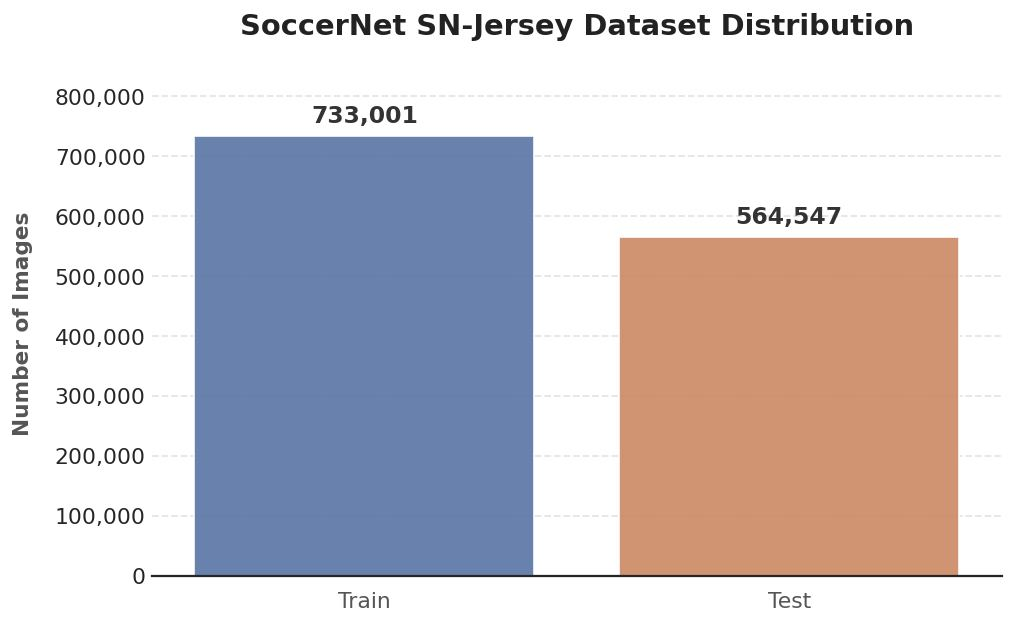
\includegraphics[width=0.75\textwidth]{figures/fig_dataset_distribution.jpg}
    \caption{Overall scale of the SoccerNet SN-Jersey dataset
    (733{,}001 training images and 564{,}547 test images).}
    \label{fig:dataset-distribution}
\end{figure}

Given the scale of the full dataset, a curated subset of \textbf{353}
player-image paths was selected for this thesis --- 269 for training and
84 for testing --- using a text file (\texttt{img\-\_path.txt}) of
representative image paths. Figure~\ref{fig:selected-images} shows the
distribution of this selected subset.

\begin{figure}[H]
    \centering
    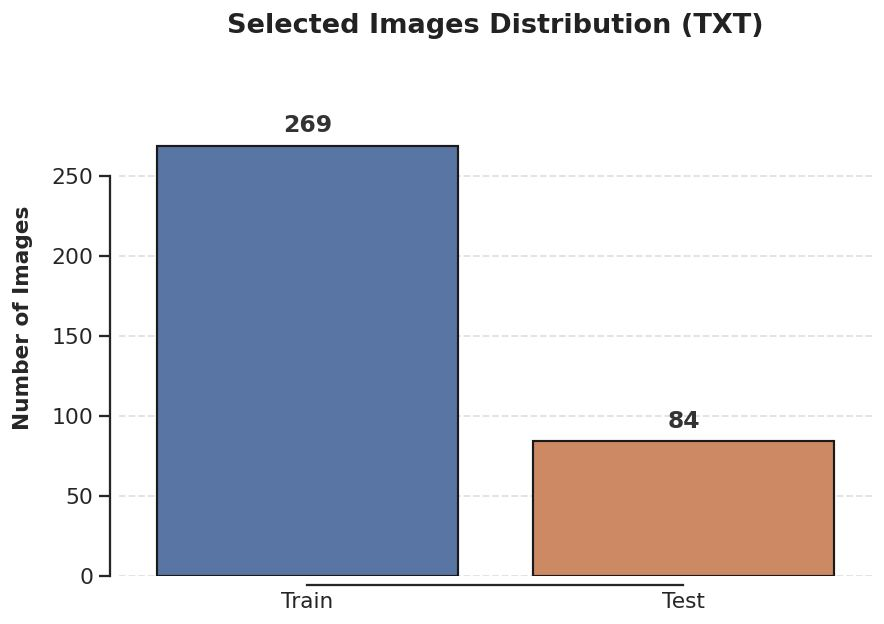
\includegraphics[width=0.75\textwidth]{figures/fig_selected_images_distribution.jpg}
    \caption{Distribution of the curated image subset (269 train / 84 test, 353 total).}
    \label{fig:selected-images}
\end{figure}

Figure~\ref{fig:dataset-demo} shows representative samples from the
subset, illustrating the variation in jersey color, player pose, and
image resolution (roughly 32$\times$101 to 70$\times$163 pixels).

\begin{figure}[H]
    \centering
    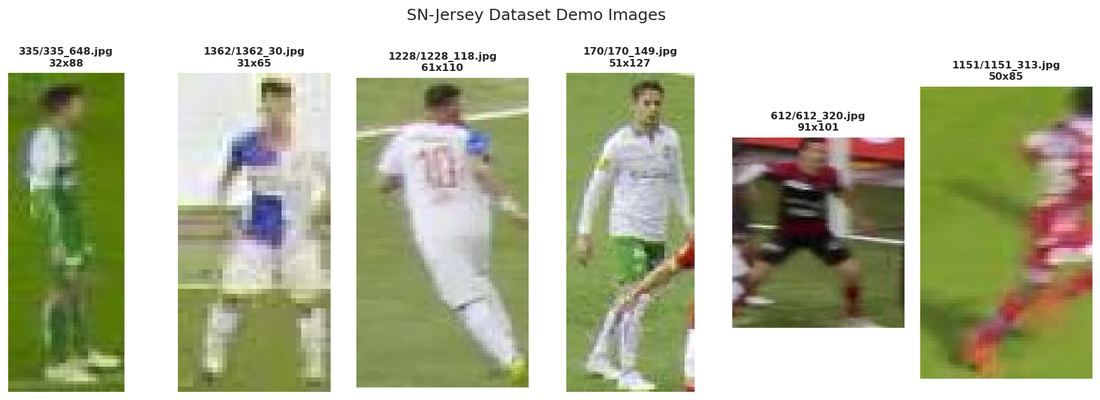
\includegraphics[width=\textwidth]{figures/fig_dataset_demo_images.jpg}
    \caption{Sample images from the SN-Jersey subset, illustrating
    variation in resolution, pose, lighting, and jersey appearance.}
    \label{fig:dataset-demo}
\end{figure}

\subsection{Broadcast Video Clips (Video Pipeline)}

The video-based pipeline is evaluated on \textbf{ten broadcast football
clips} (001.mp4 -- 010.mp4), each video clip has an approximate duration of \textbf{30 seconds}, each comprising \textbf{900 frames} at
$1920 \times 1080$ resolution and \textbf{25 fps}, sourced from the Hugging Face SoccerNet SN-PCBAS dataset (Videos 001–007) and Rutracker.org (Videos 008–010). Unlike the image dataset, these video clips include manually created
\textbf{ground-truth annotations} using CVAT. The annotations provide
per-frame player bounding boxes with track identities through
\textbf{MOT files} (in \texttt{*\_gt.txt} format), along with
\textbf{ground-truth CSV files} containing manually annotated jersey
numbers for a subset of tracked players. Therefore, evaluation of the
video pipeline is performed against verified ground-truth annotations
rather than relying solely on internal pipeline heuristics.

Figure~\ref{fig:video-dataset-samples} shows two representative
annotated frames from the video dataset, illustrating the player and
goalkeeper detection boxes with jersey-number overlays that the YOLOv5
football model and downstream OCR stage produce on typical broadcast
footage.

\begin{figure}[H]
    \centering
    \begin{subfigure}[t]{0.49\textwidth}
        \centering
        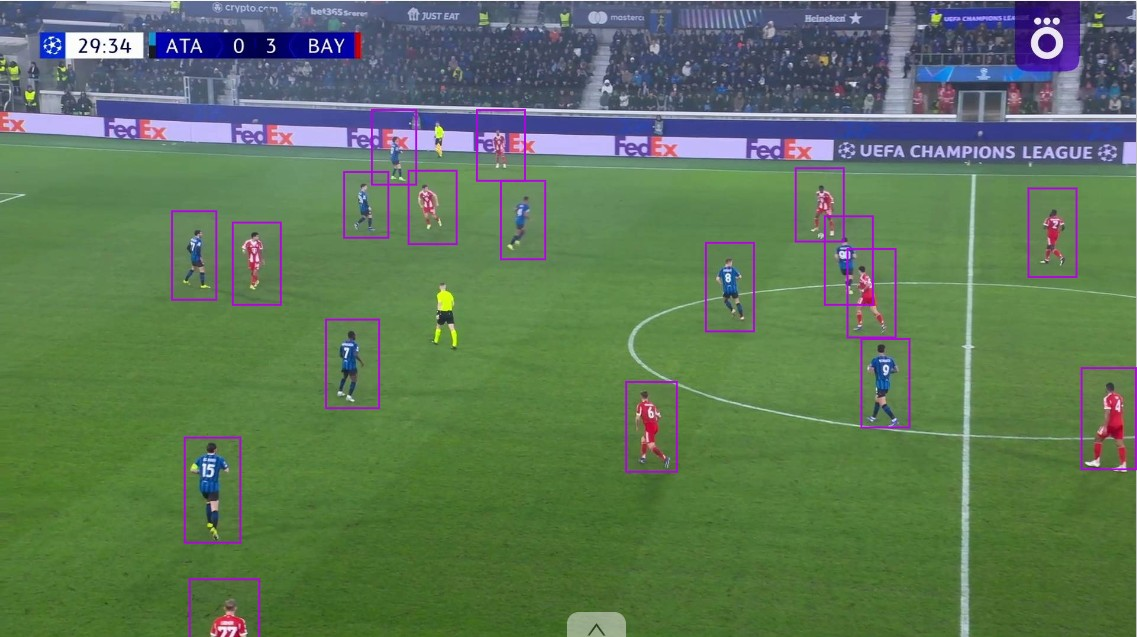
\includegraphics[width=\textwidth]{figures/fig_video_sample_frame1.jpg}
        \caption{Sample frame from a UEFA Champions League broadcast
        clip, showing detected players with jersey-number boxes across
        a wide-angle mid-field view.}
        \label{fig:video-sample-1}
    \end{subfigure}
    \hfill
    \begin{subfigure}[t]{0.49\textwidth}
        \centering
        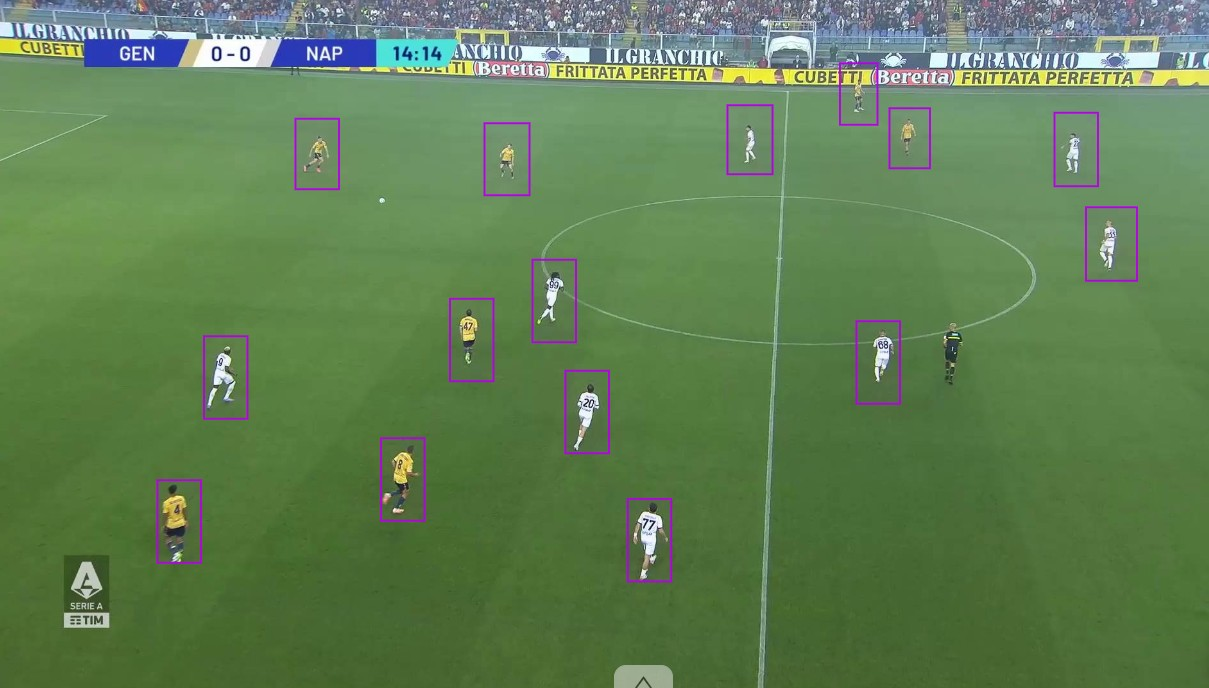
\includegraphics[width=\textwidth]{figures/fig_video_sample_frame2.jpg}
        \caption{Sample frame from a Serie A broadcast clip, showing
        detected players spread across the pitch with jersey-number
        boxes at varying distances from the camera.}
        \label{fig:video-sample-2}
    \end{subfigure}
    \caption{Representative sample frames from the ten broadcast video
    clips used to evaluate the video pipeline, illustrating the range
    of camera distances, jersey colors, and player densities present
    in the dataset.}
    \label{fig:video-dataset-samples}
\end{figure}

\section{Pre-processing and Image Enhancement}
\label{sec:preprocessing}

\subsection{Global Image Cleaning (Image Pipeline)}

Before detection or OCR, each input image is processed by
\texttt{clean\_main\_image()}, which applies the following four
operations in sequence to improve image quality for downstream
recognition.

\begin{enumerate}

    \item \textbf{Fast Non-Local Means Denoising.}
    OpenCV's \texttt{fastNlMeansDenoisingColored()} is applied to
    suppress sensor noise and compression artefacts while preserving
    sharp digit stroke edges, which are critical for OCR accuracy.

    \item \textbf{CLAHE on the LAB L-channel.}
    The image is converted to CIE LAB and Contrast Limited Adaptive
    Histogram Equalization (CLAHE) is applied to the luminance channel
    (\texttt{clipLimit=1.6}, \texttt{tileGridSize=(8,8)}). This
    enhances local contrast without distorting color information,
    improving digit visibility under uneven stadium lighting.

    \item \textbf{Bilateral Filtering.}
    A bilateral filter ($\sigma_{\text{color}}=18$,
    $\sigma_{\text{space}}=6$) smooths flat jersey regions to reduce
    residual noise while retaining sharp transitions at digit
    boundaries.

    \item \textbf{Unsharp Masking.}
    A Gaussian-blurred copy of the image is subtracted from the
    original and the resulting high-frequency detail is added back
    with a weighting coefficient, sharpening digit boundaries prior
    to OCR.
\end{enumerate}

\subsection{Crop-Level Enhancement for OCR (Image Pipeline)}

Once a jersey-number ROI is cropped, multiple enhanced variants are
generated to maximize recognition chances across diverse lighting
conditions and image orientations. The following operations are
applied to each crop:

\begin{enumerate}

    \item \textbf{Gray-World White Balance.}
    A gray-world assumption is applied to correct color casts caused
    by stadium lighting, normalizing each channel so that the mean
    pixel value across the crop is equalized.

    \item \textbf{Adaptive Gamma Correction.}
    Gamma correction is applied with $\gamma \in [0.75, 1.25]$,
    selected adaptively based on the mean luminance of the crop.
    Dark crops are brightened and over-exposed crops are dimmed to
    bring digit contrast into a consistent range.

    \item \textbf{CLAHE, Morphological Operations, and Laplacian
    Sharpening.}
    CLAHE is applied on the grayscale crop for local contrast
    enhancement. Morphological opening and closing are then used
    to remove small noise artefacts and fill minor gaps in digit
    strokes. Finally, a Laplacian sharpening filter is applied to
    further accentuate digit boundaries.

    \item \textbf{Auto-Inversion.}
    If more than 70\% of pixels in the crop are white, the image
    is automatically inverted. This ensures consistent digit
    polarity --- dark digits on a light background --- regardless
    of the original jersey color scheme.

    \item \textbf{Rotation Correction.}
    Each crop is evaluated at a set of candidate rotation angles
    $\{0^{\circ}, \pm3^{\circ}, \pm6^{\circ}\}$ to compensate
    for minor jersey tilt, and the best-scoring orientation is
    selected for OCR.
\end{enumerate}

\subsection{Torso Crop Enhancement (Video Pipeline)}

For each torso crop extracted from a detected player in the video
pipeline, four enhancement variants are independently produced and
passed to the OCR stage. Generating multiple variants increases the
likelihood that at least one representation yields a clean, readable
digit region under varying broadcast lighting conditions.

\begin{enumerate}

    \item \textbf{CLAHE on Grayscale.}
    The crop is converted to grayscale and CLAHE is applied with
    \texttt{clipLimit=3.0} to enhance local contrast, making digit
    strokes more distinguishable from the jersey background.

    \item \textbf{Bilateral Filtering followed by CLAHE.}
    A bilateral filter is first applied to smooth noise while
    preserving edges, followed by CLAHE on the resulting grayscale
    image. This combination reduces background texture interference
    before contrast enhancement.

    \item \textbf{Adaptive Thresholding with Morphological Closing.}
    Adaptive thresholding binarizes the crop using locally computed
    intensity thresholds, accommodating non-uniform illumination.
    Morphological closing is then applied to fill small gaps within
    digit strokes and connect broken contours.

    \item \textbf{Sharpening via High-Pass Kernel.}
    A $3 \times 3$ high-pass convolutional kernel is applied to
    accentuate digit edges, improving OCR performance on blurred
    or low-resolution crops.

\end{enumerate}

Torso crops smaller than $32 \times 64$ pixels are up-sampled using
cubic interpolation prior to enhancement, ensuring that digit regions
contain sufficient pixel detail for reliable OCR processing.

\section{Model Architectures and Tools}
\label{sec:models}

\subsection{Player Detection --- YOLOv8x (Image Pipeline)}

The image pipeline uses \textbf{YOLOv8x}, the largest pretrained
Ultralytics model, to detect persons in each SoccerNet image. The
\texttt{PlayerDetector} class implements a fallback cascade
(\texttt{yolov8x.pt} $\rightarrow$ \texttt{yolov8l.pt} $\rightarrow$
\ldots) to handle environments where large weights cannot be loaded.
Only detections belonging to \texttt{class\_id == 0} (COCO
\texttt{person}) with confidence $\geq 0.20$ are retained.

\subsection{Player and Role Detection --- YOLOv5 Football Model (Video Pipeline)}

The video pipeline uses a \textbf{YOLOv5} model specifically fine-tuned
on football broadcast video, loaded via
\texttt{torch.hub.load('ultralytics/yolov5', 'custom', ...)}. This model
detects four semantic classes: \textit{player}, \textit{goalkeeper},
\textit{referee}, and \textit{ball}. Using a football-specific model
significantly reduces false detections compared with a generic person
detector on broadcast footage and provides semantic role labels that
inform the temporal role voter.

\subsection{Pose Estimation --- YOLOv8x-Pose (Image Pipeline)}

A second model, \texttt{yolov8x-pose.pt}, predicts 17 COCO keypoints per
detected person. Shoulder keypoints (indices 5 and 6) and hip keypoints
(indices 11 and 12) are used to derive the torso bounding box in
\texttt{torso\_box\_from\_pose()}, with proportional margin padding
(18\% horizontal, 12\% top, 22\% bottom). When pose keypoints are
unavailable, a fallback heuristic torso box is used (central 60\%
horizontal, 30--72\% vertical of the player bounding box).

\subsection{Multi-Object Tracking --- ByteTrack (Video Pipeline)}

Player identity across frames in the video pipeline is managed by the
standalone \textbf{ByteTrack} implementation
(\texttt{BYTE\-Tracker}) cloned from the ByteTrack GitHub repository.
Detection boxes are converted to the required format using
\texttt{detections2boxes()}, and the tracker assigns persistent
\texttt{track\_id} values that are used as keys by the temporal jersey
voter. The tracker configuration uses \texttt{track\-\_thresh=0.25},
\texttt{track\-\_buffer=30}, and \texttt{match\_thresh=0.8}.

\subsection{OCR Engine --- Multi-Variant EasyOCR (Image Pipeline)}

The image pipeline uses \textbf{EasyOCR} as its recognition backend,
restricted to the digit allowlist \texttt{"0123456789"} with a maximum
of two recognized characters, consistent with valid football jersey
numbers (1--99). Rather than invoking EasyOCR once per crop, the image
pipeline wraps it in the multi-variant strategy described in
Section~\ref{sec:multi-variant-ocr}, which evaluates multiple
enhancement variants, zoom levels, and binarization strategies before
selecting the highest-scoring candidate.

\subsection{OCR Engine --- PARSeq with EasyOCR Fallback (Video Pipeline)}

The video pipeline uses the \texttt{JerseyRecognizer} class, which
attempts to load a pretrained \textbf{PARSeq} scene-text recognition
model \cite{bautista2022parseq} (via \texttt{torch.hub} from the
\texttt{baudm/parseq} repository) at start-up. PARSeq is an
attention-based sequence model that decodes the digit string directly
from the enhanced torso crop without an explicit character-segmentation
step, and its confidence score is taken as the mean token probability
of the decoded sequence. If PARSeq cannot be loaded in the runtime
environment --- for example, because the required \texttt{strhub}
dependency is unavailable --- \texttt{JerseyRecognizer} automatically
falls back to \textbf{EasyOCR} for the remainder of the run, restricted
to the same digit allowlist as the image pipeline. This fallback is a
load-time decision made once when the recognizer is instantiated, and
the active backend is logged for every video so that the source of
each prediction remains traceable; Figure~\ref{fig:video-step6-ocr} in
Section~\ref{sec:video-visual-walkthrough} shows one such prediction
card in which the EasyOCR fallback was the active backend, confirming
that the fallback path is genuinely exercised in practice rather than
being purely theoretical.

\subsection{Legibility Classifier --- ResNet-18 (Image Pipeline)}

A binary \textbf{legibility classifier} based on \textbf{ResNet-18}
is trained to predict whether a jersey-number crop is \textit{legible}
(label 1) or \textit{illegible} (label 0). The final fully connected
layer is replaced by \texttt{nn.Sequential(nn.Dropout(0.25),
nn.Linear(num\_features, 1))}, producing a single logit. Weak labels
are derived automatically: a crop is labeled \textit{legible} if the
multi-variant OCR returned at least one digit with confidence
$\geq 0.55$, and \textit{illegible} otherwise.

\section{Algorithmic and Mathematical Formulation of Core Models}
\label{sec:algorithm-math}

This section presents the algorithmic and mathematical formulation of
the core models introduced in Section~\ref{sec:models}, complementing
their conceptual descriptions with the underlying objective functions
and update rules that govern their behavior.

\subsection{YOLOv8 / YOLOv5 Detection Objective}

Both the YOLOv8x detector (image pipeline) and the YOLOv5 football
detector (video pipeline) are single-stage detectors trained to
minimize a composite loss over a dense grid of candidate boxes. For a
predicted box $\hat{b} = (\hat{x}, \hat{y}, \hat{w}, \hat{h})$ matched
to a ground-truth box $b = (x, y, w, h)$, the localization term is a
Complete-IoU (CIoU) loss,
\begin{equation}
    \mathcal{L}_{\text{CIoU}} = 1 - \text{IoU}(\hat{b}, b)
    + \frac{\rho^2(\hat{b}, b)}{c^2} + \alpha v,
    \label{eq:ciou}
\end{equation}
where $\rho(\hat{b}, b)$ is the Euclidean distance between box centers,
$c$ is the diagonal length of the smallest enclosing box, $v$ measures
aspect-ratio consistency, and $\alpha$ weights $v$ relative to the
distance term. The total detection loss combines this localization
term with a binary cross-entropy objectness loss
$\mathcal{L}_{\text{obj}}$ and a classification loss
$\mathcal{L}_{\text{cls}}$:
\begin{equation}
    \mathcal{L}_{\text{det}} = \lambda_{\text{box}}\mathcal{L}_{\text{CIoU}}
    + \lambda_{\text{obj}}\mathcal{L}_{\text{obj}}
    + \lambda_{\text{cls}}\mathcal{L}_{\text{cls}}.
    \label{eq:yolo-loss}
\end{equation}
Both detectors used in this thesis are applied with pretrained weights
at inference time only; Equations~\ref{eq:ciou}--\ref{eq:yolo-loss}
describe the objective used during their original training and are
included here for completeness, since they determine the confidence
calibration and localization precision that Chapter~\ref{ch:results}
builds upon.

\subsection{Pose Keypoint Localization}

YOLOv8x-Pose predicts, for each detected person, a set of 17 keypoints
$\{(\hat{p}_k, v_k)\}_{k=1}^{17}$, where $\hat{p}_k = (\hat{x}_k,
\hat{y}_k)$ is the predicted image location of keypoint $k$ and $v_k$
is a visibility/confidence score. The torso box used in this thesis is
derived deterministically from four of these keypoints --- left/right
shoulder ($k{=}5,6$) and left/right hip ($k{=}11,12$) --- as
\begin{equation}
    x_{\min} = \min_k \hat{x}_k, \quad
    x_{\max} = \max_k \hat{x}_k, \quad
    y_{\text{top}} = \min(\hat{y}_5, \hat{y}_6), \quad
    y_{\text{bot}} = \max(\hat{y}_{11}, \hat{y}_{12}),
    \label{eq:torso-box}
\end{equation}
followed by proportional margin expansion of 18\% horizontally, 12\%
at the top, and 22\% at the bottom, as summarized in
Table~\ref{tab:hp-detection}. When keypoints are unavailable, the
fallback heuristic torso box described in
Section~\ref{sec:models} is used instead of
Equation~\ref{eq:torso-box}.

\subsection{ByteTrack Association}

ByteTrack maintains, for each active track $i$, a Kalman filter state
$s_i = (x_i, y_i, \gamma_i, h_i, \dot{x}_i, \dot{y}_i, \dot{\gamma}_i,
\dot{h}_i)$ representing bounding-box center, aspect ratio, height, and
their velocities. At each frame, the predict step propagates the state
forward under a constant-velocity motion model, and the update step
corrects it using the associated detection. Association between
predicted track boxes and detection boxes is formulated as a linear
assignment problem over an IoU-based cost matrix,
\begin{equation}
    C_{ij} = 1 - \text{IoU}(\hat{b}_i, d_j),
    \label{eq:bytetrack-cost}
    \end{equation}
solved with the Hungarian algorithm subject to the
\texttt{match\_thresh} constraint in Table~\ref{tab:hp-bytetrack}.
ByteTrack's key departure from earlier trackers is a second association
pass: detections above the confidence threshold are matched first, and
any tracks left unmatched are given a second opportunity to match
against low-confidence detections that would otherwise be discarded,
which is what allows the tracker to recover from brief occlusions
without spawning a new identity.

\subsection{ResNet-18 Legibility Classifier Objective}

The legibility classifier produces a single logit $z$ for an input crop
$x$, and is trained with a class-weighted binary cross-entropy loss,
\begin{equation}
    \mathcal{L}_{\text{BCE}}(z, y) = -\big[w_{\text{pos}}\, y \log
    \sigma(z) + (1-y) \log (1-\sigma(z))\big],
    \label{eq:bce}
\end{equation}
where $y \in \{0, 1\}$ is the weak legibility label, $\sigma(\cdot)$ is
the logistic sigmoid, and $w_{\text{pos}} = N_{\text{neg}} /
N_{\text{pos}}$ is the positive class weight introduced in
Section~\ref{sec:models} to compensate for the natural imbalance
between legible and illegible crops. The residual connections in the
ResNet-18 backbone itself follow the identity-mapping formulation
$y = \mathcal{F}(x, \{W_i\}) + x$, where $\mathcal{F}$ is the learned
residual function of a block and the identity shortcut $x$ allows
gradients to propagate directly through the network, which is what
makes deep backbones of this kind trainable in the first place
\cite{he2016resnet}.

\subsection{PARSeq Sequence Modeling (Video Pipeline)}

PARSeq treats jersey digit recognition as a sequence generation problem
over the digit alphabet, using a permutation language modeling
objective during pretraining: for a target sequence of length $T$ and a
permutation $z$ of the position indices $\{1, \dots, T\}$, the model is
trained to maximize
\begin{equation}
    \log p_\theta(y \mid x) = \sum_{t=1}^{T} \log p_\theta\big(y_{z_t}
    \mid y_{z_{<t}}, x\big),
    \label{eq:parseq}
\end{equation}
where $x$ is the input crop and $y_{z_{<t}}$ denotes the target tokens
preceding position $z_t$ under permutation $z$. Because this objective
is evaluated over multiple permutations rather than a single fixed
left-to-right order, the same trained model supports both
autoregressive and parallel (non-autoregressive) decoding at inference
time \cite{bautista2022parseq}. At inference, the recognizer in this
thesis takes the arg-max token at each position and reports the mean
per-token probability as the confidence score used by the temporal
jersey voter in Section~\ref{sec:temporal-voting}.

\subsection{Multi-Variant OCR Candidate Scoring (Image Pipeline)}

The multi-variant OCR pipeline described in
Section~\ref{sec:multi-variant-ocr} produces a set of candidate digit
strings $\{(d_k, c_k, \tau_k)\}$, where $c_k$ is the OCR confidence and
$\tau_k$ is a tag identifying the generating method. The final
prediction is the candidate maximizing
\begin{equation}
    \text{score}(d_k) = c_k + \beta(\tau_k) + \ell(|d_k|),
    \label{eq:ocr-score}
\end{equation}
where $\beta(\tau_k)$ is the method bonus (rewarding
binarization-based candidates) and $\ell(|d_k|)$ is the length bonus
that slightly favors two-digit predictions, both listed numerically in
Table~\ref{tab:hp-ocr}.

\subsection{Temporal Voting (Video Pipeline)}

For a track with observation history $\{(n_t, c_t)\}_{t=1}^{T}$ within
the sliding window (jersey number and confidence at frame $t$), the
temporal jersey voter accumulates confidence-weighted support for each
candidate number,
\begin{equation}
    w(n) = \sum_{t : n_t = n} c_t,
    \label{eq:temporal-vote}
\end{equation}
and reports $n^{*} = \arg\max_n w(n)$ as the consensus jersey number for
that track once at least \texttt{min\_votes} valid observations have
been accumulated (Table~\ref{tab:hp-voters}). The temporal role voter
for referee identification follows the same weighted-majority principle
but over binary class labels rather than digit strings.

\section{Multi-Variant OCR Pipeline (Image Pipeline)}
\label{sec:multi-variant-ocr}

The core OCR logic is implemented in \texttt{ocr\_digits\_strict()},
which combines several independent recognition strategies and selects the
most reliable result through the following stages:

\begin{enumerate}
    \item \textbf{Seed pass:} A white-balanced, CLAHE-enhanced crop is
    passed through EasyOCR as an initial estimate.

    \item \textbf{Multi-variant dynamic-zoom OCR:} Each enhancement
    variant is evaluated at zoom levels
    \texttt{[96, 128, 192, 256]} pixels height. Search stops early when
    a valid 1--2 digit result with confidence $\geq 0.92$ is found;
    otherwise, the highest-scoring result across all variants and scales
    is retained.

    \item \textbf{Per-digit isolation:} Six binarization strategies
    (Otsu, inverted Otsu, adaptive, inverted adaptive, morphological
    opening, morphological closing) extract candidate digit bounding
    boxes from connected components; each isolated digit is
    independently re-OCR'd and results are concatenated.

    \item \textbf{Projection-split OCR:} The vertical projection profile
    of the binarized crop is analyzed for a central ``valley''; if
    found, the crop is split and each half is independently OCR'd as a
    separate digit.

    \item \textbf{Candidate scoring:} All candidates are scored using
    $\text{score} = \text{conf} + \text{method\_bonus} +
    \text{LENGTH\_BONUS}$, where \texttt{method\_bonus} rewards
    binarization-based candidates and \texttt{LENGTH\_BONUS} gives a
    small preference to two-digit results.

    \item \textbf{Shape-based digit refinement:} The selected digit
    string is refined by (a) counting enclosed contour holes to
    disambiguate 0/6/8/9, and (b) comparing top-row ink density with
    central-column density to distinguish the digits 1 and 7.
\end{enumerate}

\section{Temporal Jersey Voting Mechanism (Video Pipeline)}
\label{sec:temporal-voting}

Because a single video frame frequently yields no usable OCR result,
the video pipeline implements a \textbf{temporal jersey voting} mechanism
via the \texttt{Temporal\-Jersey\-Voter} class. For each tracked player
(identified by \texttt{track\_id}):

\begin{enumerate}
    \item OCR is run on every frame in which the player's torso crop
    meets minimum quality criteria (\mbox{\texttt{MIN\_CROP\_HEIGHT\_FOR\_OCR}
    = 40} pixels).
    \item Per-frame results are stored in a sliding window of the most
    recent \texttt{window=60} observations, with a minimum confidence
    of \texttt{min\-\_conf=0.25} and at least \texttt{min\-\_votes=3} valid
    observations required before a consensus is reported.
    \item The most frequently occurring valid digit string within the
    window is returned as the player's current jersey number.
\end{enumerate}

\section{Temporal Role Voter (Video Pipeline)}

To avoid wasting OCR resources on match officials, a
\texttt{Temporal\-Role\-Voter} classifies each track as either
\textit{player} or \textit{referee} based on the semantic class labels
assigned by the YOLOv5 football detection model. Over a sliding window
of the last 20 observations, a track is locked as \textit{referee} when
the referee class constitutes at least 60\% of its observed labels and
at least 5 observations have been accumulated.

\section{Ground-Truth Evaluation (Video Pipeline)}
\label{sec:gt-eval}

The video pipeline is evaluated using the
\texttt{GT\-Tracking\-And\-Jersey\-Eval} class, which:

\begin{itemize}[noitemsep]
    \item Loads per-video MOT ground-truth files and manually annotated
    jersey-number CSV files.
    \item Matches predicted tracks to ground-truth tracks frame by frame
    using an IoU threshold of 0.30.
    \item Computes standard multi-object tracking metrics: tracking
    accuracy (MOTA equivalent), IDF1, ID precision, track recall, and
    ID switches.
    \item Computes OCR accuracy by comparing the temporal-voted jersey
    number for each matched track against the ground-truth jersey number.
\end{itemize}

\section{Evaluation Metrics}
\label{sec:eval-metrics}

The following metrics are used to quantify system performance:

\begin{itemize}[noitemsep]
    \item \textbf{Player-level accuracy (image pipeline):} The mode of
    per-crop OCR predictions per player folder is compared against the
    SoccerNet ground-truth jersey number.
    \item \textbf{Tracking accuracy (video pipeline):} Fraction of
    correctly assigned track-frame pairs, based on IoU matching with
    ground-truth boxes.
    \item \textbf{IDF1:} The IDSW-sensitive harmonic mean of
    identification precision and recall.
    \item \textbf{GT OCR accuracy:} Fraction of ground-truth-annotated
    tracks for which the temporal-voted jersey number matches the
    annotated number.
    \item \textbf{Overall accuracy:} Combined measure accounting for
    both tracking and jersey recognition correctness.
    \item \textbf{Raw vs.\ temporal-voting OCR accuracy:} Comparison
    of per-frame raw OCR predictions against temporally voted
    predictions on the same evaluation rows.
    \item \textbf{Legibility classifier metrics:} Validation accuracy,
    ROC-AUC, average precision, and per-class accuracy.
\end{itemize}

\section{Hyperparameter Configuration}
\label{sec:hyperparameters}

This section consolidates all configurable hyperparameters used across
both pipelines. Well-chosen hyperparameters are essential because they
directly control the balance between detection sensitivity and false
alarm rate, the OCR confidence thresholds that determine when a reading
is accepted, the temporal window lengths that govern how much historical
evidence is aggregated, and the training dynamics of the legibility
classifier. Each group of parameters is discussed below.

\subsection{Detection and Localization Hyperparameters}

Table~\ref{tab:hp-detection} lists the threshold and margin values
governing player detection, pose estimation, and torso/ROI localization.

\begin{table}[H]
    \centering
    \caption{Detection and localization hyperparameters for both pipelines.}
    \label{tab:hp-detection}
    \resizebox{\textwidth}{!}{%
    \begin{tabular}{@{}p{4cm}p{3.5cm}p{3.5cm}p{4cm}@{}}
        \toprule
        \textbf{Parameter} & \textbf{Image Pipeline} & \textbf{Video Pipeline} & \textbf{Rationale} \\
        \midrule
        Detection model & YOLOv8x & YOLOv5 (football) & Domain specificity \\
        Detection confidence & 0.20 & 0.25 & Low threshold to recover partial detections \\
        Input size (inference) & Native & 1280 px (long side) & Preserves small player detail in HD video \\
        Pose keypoints used & Shoulders (5,6), Hips (11,12) & N/A & Cover jersey digit region \\
        Torso horizontal margin & $\pm$18\% of torso width & 20--80\% of box width & Avoids arm occlusion \\
        Torso top margin & $-$12\% of torso height & 20\% of box height & Includes collar digits \\
        Torso bottom margin & $+$22\% of torso height & 55\% of box height & Excludes shorts numbers \\
        Min crop size (OCR) & N/A & $30\times40$ px & Prevents degenerate crops \\
        Min crop height (OCR) & N/A & 40 px & Below this, OCR is unreliable \\
        \bottomrule
    \end{tabular}}
\end{table}

\subsection{OCR Pipeline Hyperparameters}

Table~\ref{tab:hp-ocr} lists the parameters controlling the
multi-variant OCR engine used in both pipelines.

\begin{table}[H]
    \centering
    \caption{OCR pipeline hyperparameters.}
    \label{tab:hp-ocr}
    \resizebox{\textwidth}{!}{%
    \begin{tabular}{@{}p{4.5cm}p{4.5cm}p{6cm}@{}}
        \toprule
        \textbf{Parameter} & \textbf{Value} & \textbf{Description} \\
        \midrule
        Digit allowlist & \texttt{"0123456789"} & Limits OCR output (EasyOCR or PARSeq) to digit characters only \\
        Max recognized characters & 2 & Jersey numbers have at most 2 digits \\
        Valid jersey range & $[1, 99]$ & Rejects out-of-range OCR outputs \\
        Zoom target heights (image) & 96, 128, 192, 256 px & Dynamic upscaling steps \\
        Early-stop confidence (image) & 0.92 & Stops zoom loop when high-confidence result is found \\
        Max zoom attempts (image) & 6 & Prevents excessive inference time per crop \\
        Min OCR confidence (video) & 0.25 & Minimum confidence to feed into temporal voter \\
        Binarization variants (image) & 6 (Otsu, adaptive, morphological $\times$2 each) & Cover diverse lighting conditions \\
        Rotation candidates (image) & $\{0^{\circ}, \pm3^{\circ}, \pm6^{\circ}\}$ & Corrects minor jersey tilt \\
        Method bonus (binarization) & +0.05 confidence & Prioritizes isolation-based candidates \\
        Length bonus (2-digit) & +0.04 confidence & Slightly favours two-digit predictions \\
        \bottomrule
    \end{tabular}}
\end{table}

\noindent The zoom strategy is critical because jersey digits in the
SN-Jersey dataset often occupy fewer than $20\times20$ pixels at native
resolution, which is below the reliable range of EasyOCR's text detector.
Upscaling to 128--256 px target height before inference has been observed
empirically to substantially improve detection of single digits in
particular. The early-stop mechanism at 0.92 confidence prevents
unnecessary additional zoom iterations when a clean reading is already
available, reducing per-crop inference time.

\subsection{Legibility Classifier Hyperparameters}

The ResNet-18 legibility classifier is trained with the hyperparameter
configuration shown in Table~\ref{tab:hp-legibility}. The choice of
ResNet-18 balances training speed, model size, and representational
capacity for the binary legibility task: with only $\sim$11 million
parameters, it trains to convergence in 20 epochs on a single P100
GPU in a few minutes.

\begin{table}[H]
    \centering
    \caption{Legibility classifier training hyperparameters.}
    \label{tab:hp-legibility}
    \resizebox{\textwidth}{!}{%
    \begin{tabular}{@{}p{5cm}p{4cm}p{6cm}@{}}
        \toprule
        \textbf{Hyperparameter} & \textbf{Value} & \textbf{Description} \\
        \midrule
        Backbone & ResNet-18 & Pretrained on ImageNet \\
        Final layer & Dropout(0.25) $\rightarrow$ Linear($\text{features}$, 1) & Single logit output \\
        Input resolution & $96 \times 96$ px (RGB) & Sufficient for digit texture features \\
        Batch size & 64 & Stable gradient estimates \\
        Training epochs & 20 & Best val accuracy stabilizes by epoch 5--6 \\
        Optimizer & AdamW & Weight decay decoupled from gradient \\
        Base learning rate & $2 \times 10^{-4}$ & Suitable for fine-tuning pretrained CNN \\
        Weight decay & $1 \times 10^{-4}$ & L2 regularization \\
        Loss function & BCEWithLogitsLoss & Numerically stable for binary classification \\
        Positive class weight & $N_{\text{neg}} / N_{\text{pos}}$ & Compensates for legibility imbalance \\
        LR scheduler & ReduceLROnPlateau & Factor 0.6, patience 2 epochs \\
        Scheduler monitor & Validation loss & Reduces LR when val loss plateaus \\
        Train/val split & 80 / 20 stratified & Random state 42 \\
        Legibility label threshold & 0.55 OCR confidence & Crops above this confidence are labeled legible \\
        Augmentation (train) & Color jitter ($p{=}0.5$), rotation ($\pm5^{\circ}$) & Increases crop diversity \\
        Normalization & ImageNet mean/std & Matches pretrained backbone statistics \\
        \bottomrule
    \end{tabular}}
\end{table}

\subsection{ByteTrack Multi-Object Tracking Hyperparameters}

Table~\ref{tab:hp-bytetrack} lists the ByteTrack configuration parameters
used in the video pipeline.

\begin{table}[H]
    \centering
    \caption{ByteTrack tracker hyperparameters used in the video pipeline.}
    \label{tab:hp-bytetrack}
    \resizebox{0.85\textwidth}{!}{%
    \begin{tabular}{@{}p{3.5cm}p{2cm}p{8cm}@{}}
        \toprule
        \textbf{Parameter} & \textbf{Value} & \textbf{Description} \\
        \midrule
        \texttt{track\_thresh} & 0.25 & Minimum detection confidence to initiate a new track \\
        \texttt{track\_buffer} & 30 frames & Number of frames a lost track is kept alive in the buffer \\
        \texttt{match\_thresh} & 0.80 & IoU threshold for accepting a detection-to-track association \\
        Frame rate & 25 fps & Matches the broadcast clip frame rate \\
        \bottomrule
    \end{tabular}}
\end{table}

\noindent A \texttt{track\_buffer} of 30 frames (1.2 seconds at 25 fps)
is sufficient to recover most short occlusion events caused by players
crossing in front of each other. Setting \texttt{match\_thresh} to 0.80
is deliberately conservative to avoid incorrect identity switches
between nearby players, which would corrupt the temporal jersey voting
history for both tracks.

\subsection{Temporal Voter Hyperparameters}

Table~\ref{tab:hp-voters} consolidates the hyperparameters for both the
temporal role voter (referee classification) and the temporal jersey
voter (jersey number aggregation).

\begin{table}[H]
    \centering
    \caption{Temporal voter hyperparameters for referee detection and jersey number aggregation.}
    \label{tab:hp-voters}
    \resizebox{\textwidth}{!}{%
    \begin{tabular}{@{}p{2.5cm}p{3.5cm}p{3cm}p{6cm}@{}}
        \toprule
        \textbf{Voter} & \textbf{Parameter} & \textbf{Value} & \textbf{Rationale} \\
        \midrule
        Role voter & Window size & 20 frames & Short window to quickly lock in referee status \\
        Role voter & Referee class ratio & 0.60 & Majority, not unanimity, required \\
        Role voter & Min observations & 5 & Avoids premature locking from single-frame noise \\
        \midrule
        Jersey voter & Window size & 60 frames (2.4 s) & Long window to accumulate sufficient OCR evidence \\
        Jersey voter & Min OCR confidence & 0.25 & Low threshold; voter handles noise through plurality \\
        Jersey voter & Min valid votes & 3 & Prevents decisions from single-frame outliers \\
        \bottomrule
    \end{tabular}}
\end{table}

\noindent The 60-frame jersey voter window is a key design choice.
Football players are rarely stationary, so a short window would
frequently yield too few valid OCR readings to form a reliable majority.
A 60-frame window corresponds to 2.4 seconds of broadcast video ---
long enough for a player to appear in at least several clearly visible
poses, but short enough to remain responsive to jersey-number
corrections (e.g.\ if the initial window contained an incorrect reading
caused by a partially occluded frame).

\section{Visual Process Walkthrough --- Image Pipeline}
\label{sec:image-visual-walkthrough}

To make the abstract module descriptions above concrete, this section
presents an input/output visual walkthrough of every major processing
stage in the image pipeline, generated directly from the implementation
on a representative SoccerNet sample.

\begin{figure}[H]
    \centering
    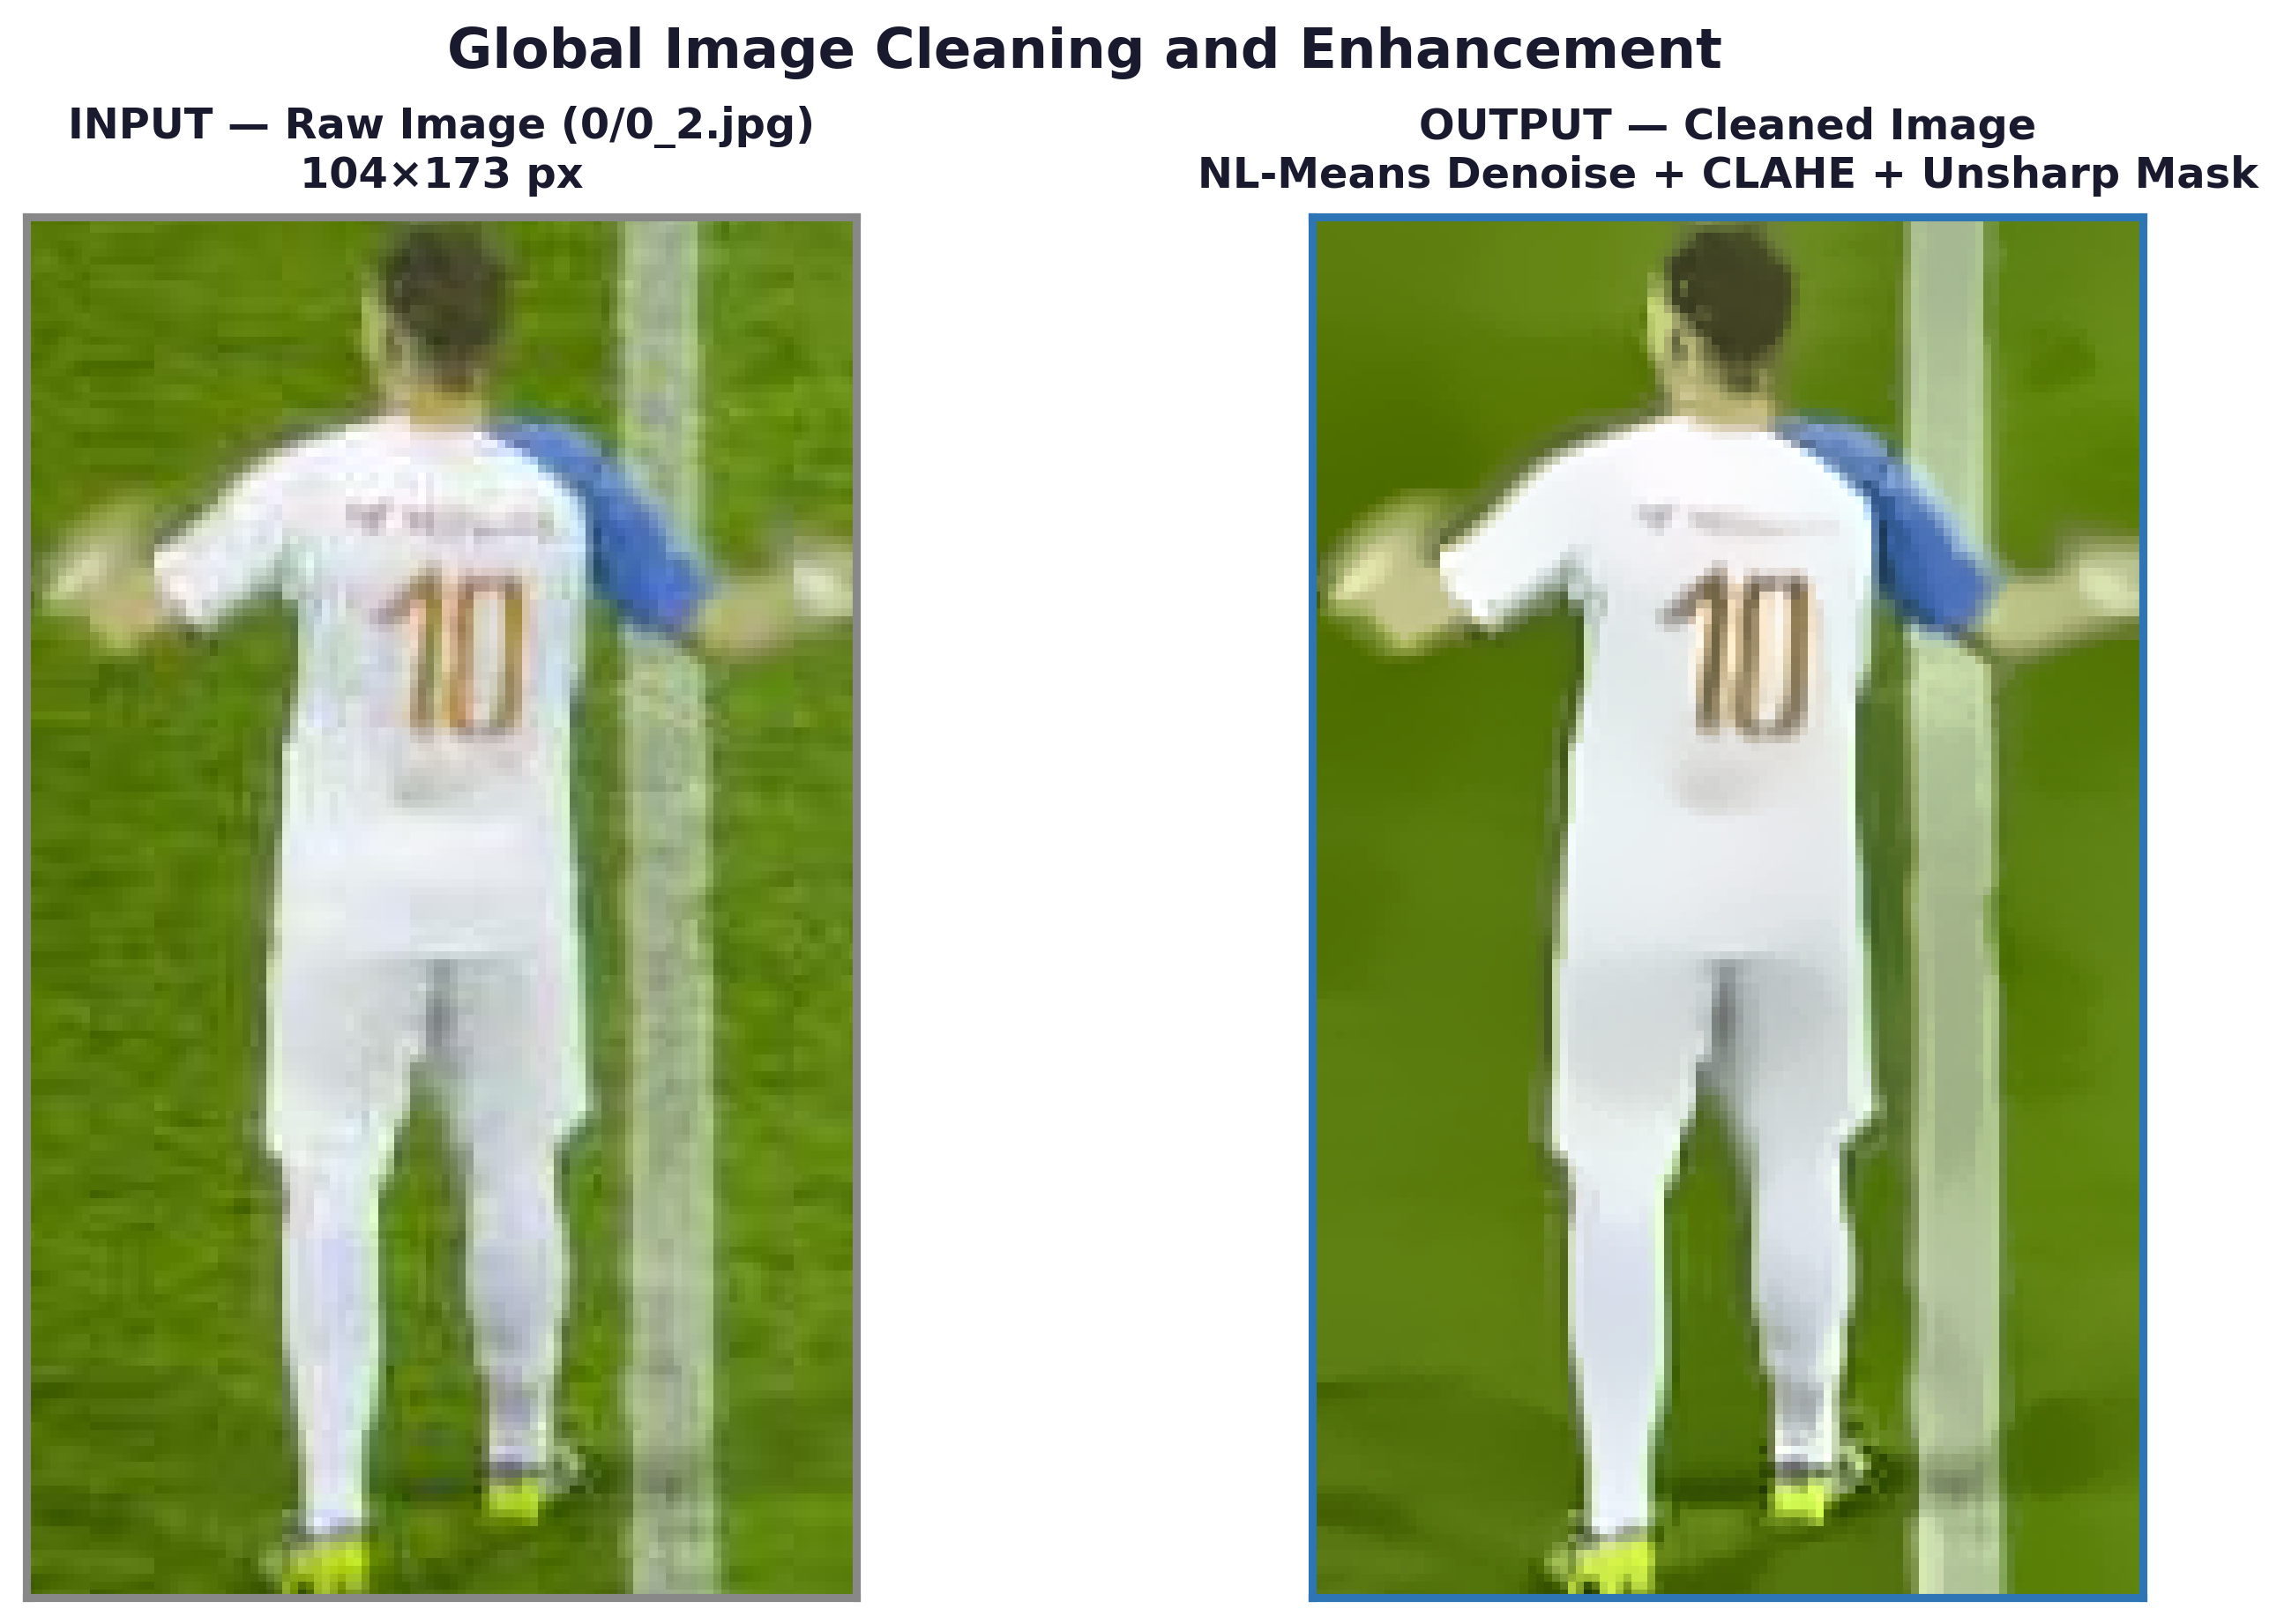
\includegraphics[width=0.85\textwidth]{figures/steps_image/fig_global_cleaning.png}
    \caption{Global image cleaning (Section~\ref{sec:preprocessing}).
    The raw input image is processed by \texttt{clean\_main\_image()},
    which applies non-local-means denoising, CLAHE contrast
    enhancement, and unsharp masking to produce the cleaned output image
    used for downstream detection.}
    \label{fig:step-img-cleaning}
\end{figure}

\begin{figure}[H]
    \centering
    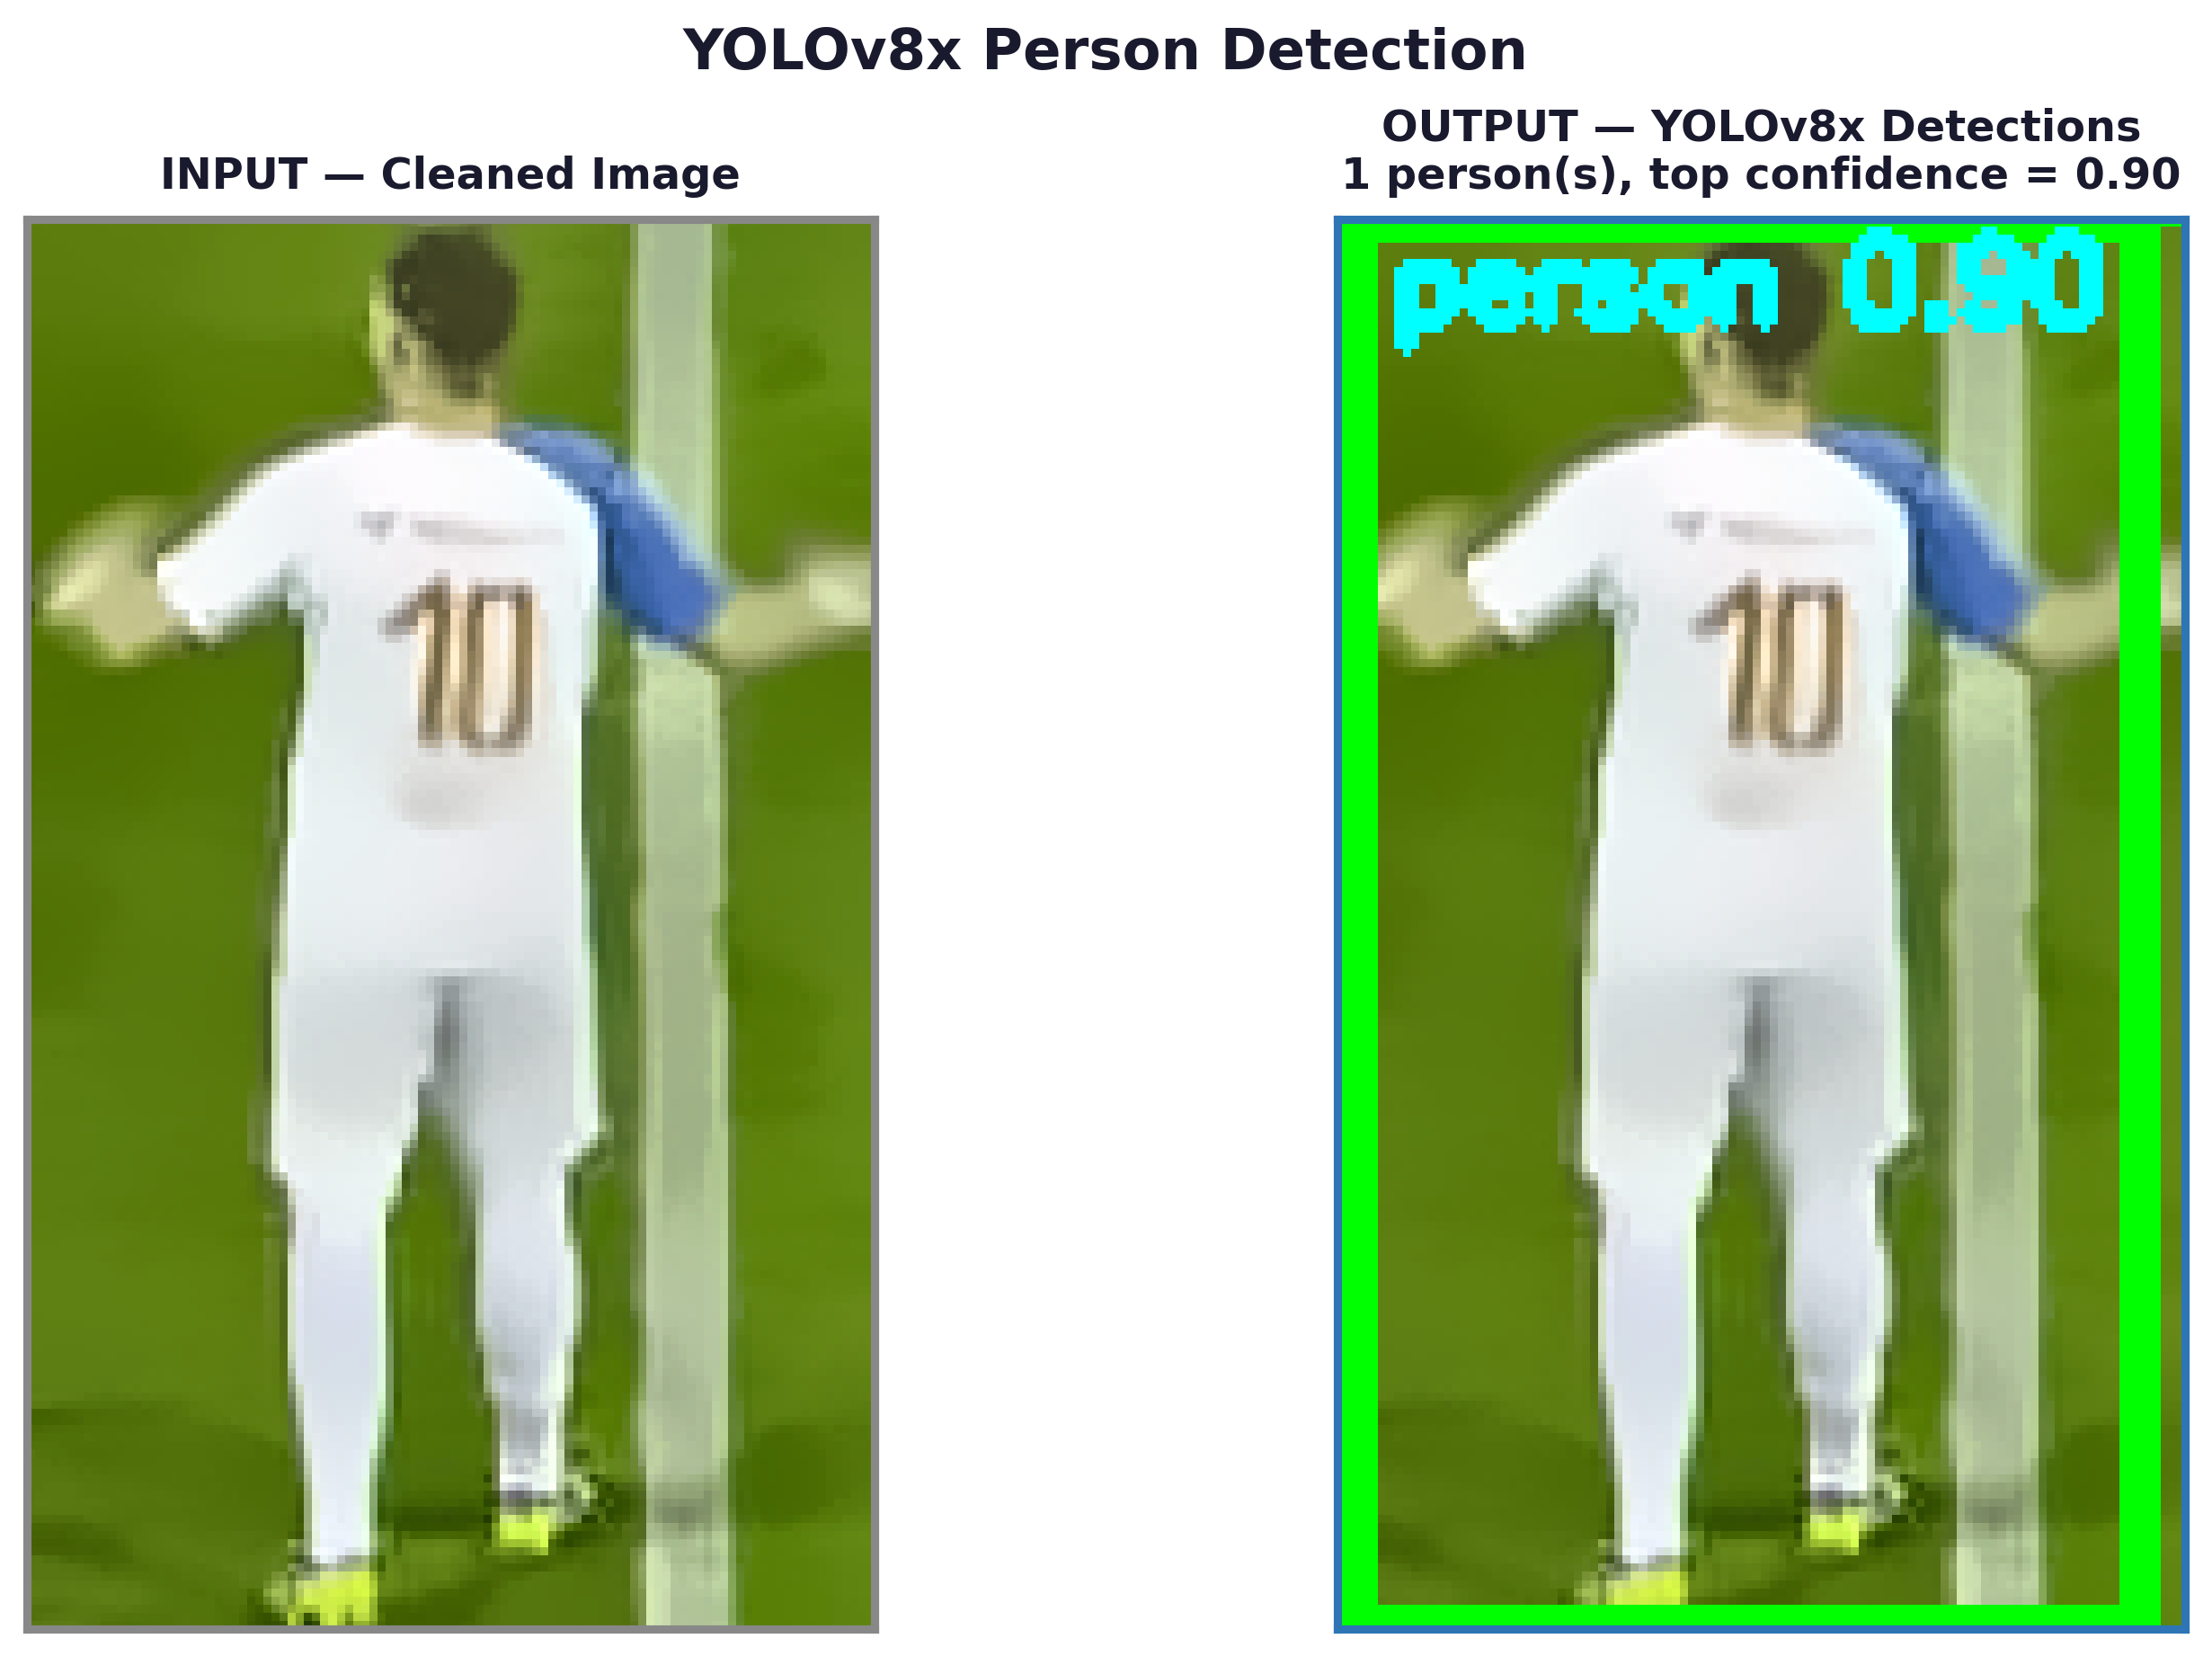
\includegraphics[width=0.85\textwidth]{figures/steps_image/fig_person_detection.png}
    \caption{YOLOv8x person detection (Section~\ref{sec:models}). The
    cleaned image is passed to the \texttt{PlayerDetector}, which
    localizes each person with a confidence score; in this example, one
    person is detected with a top confidence of 0.90.}
    \label{fig:step-img-detection}
\end{figure}

\begin{figure}[H]
    \centering
    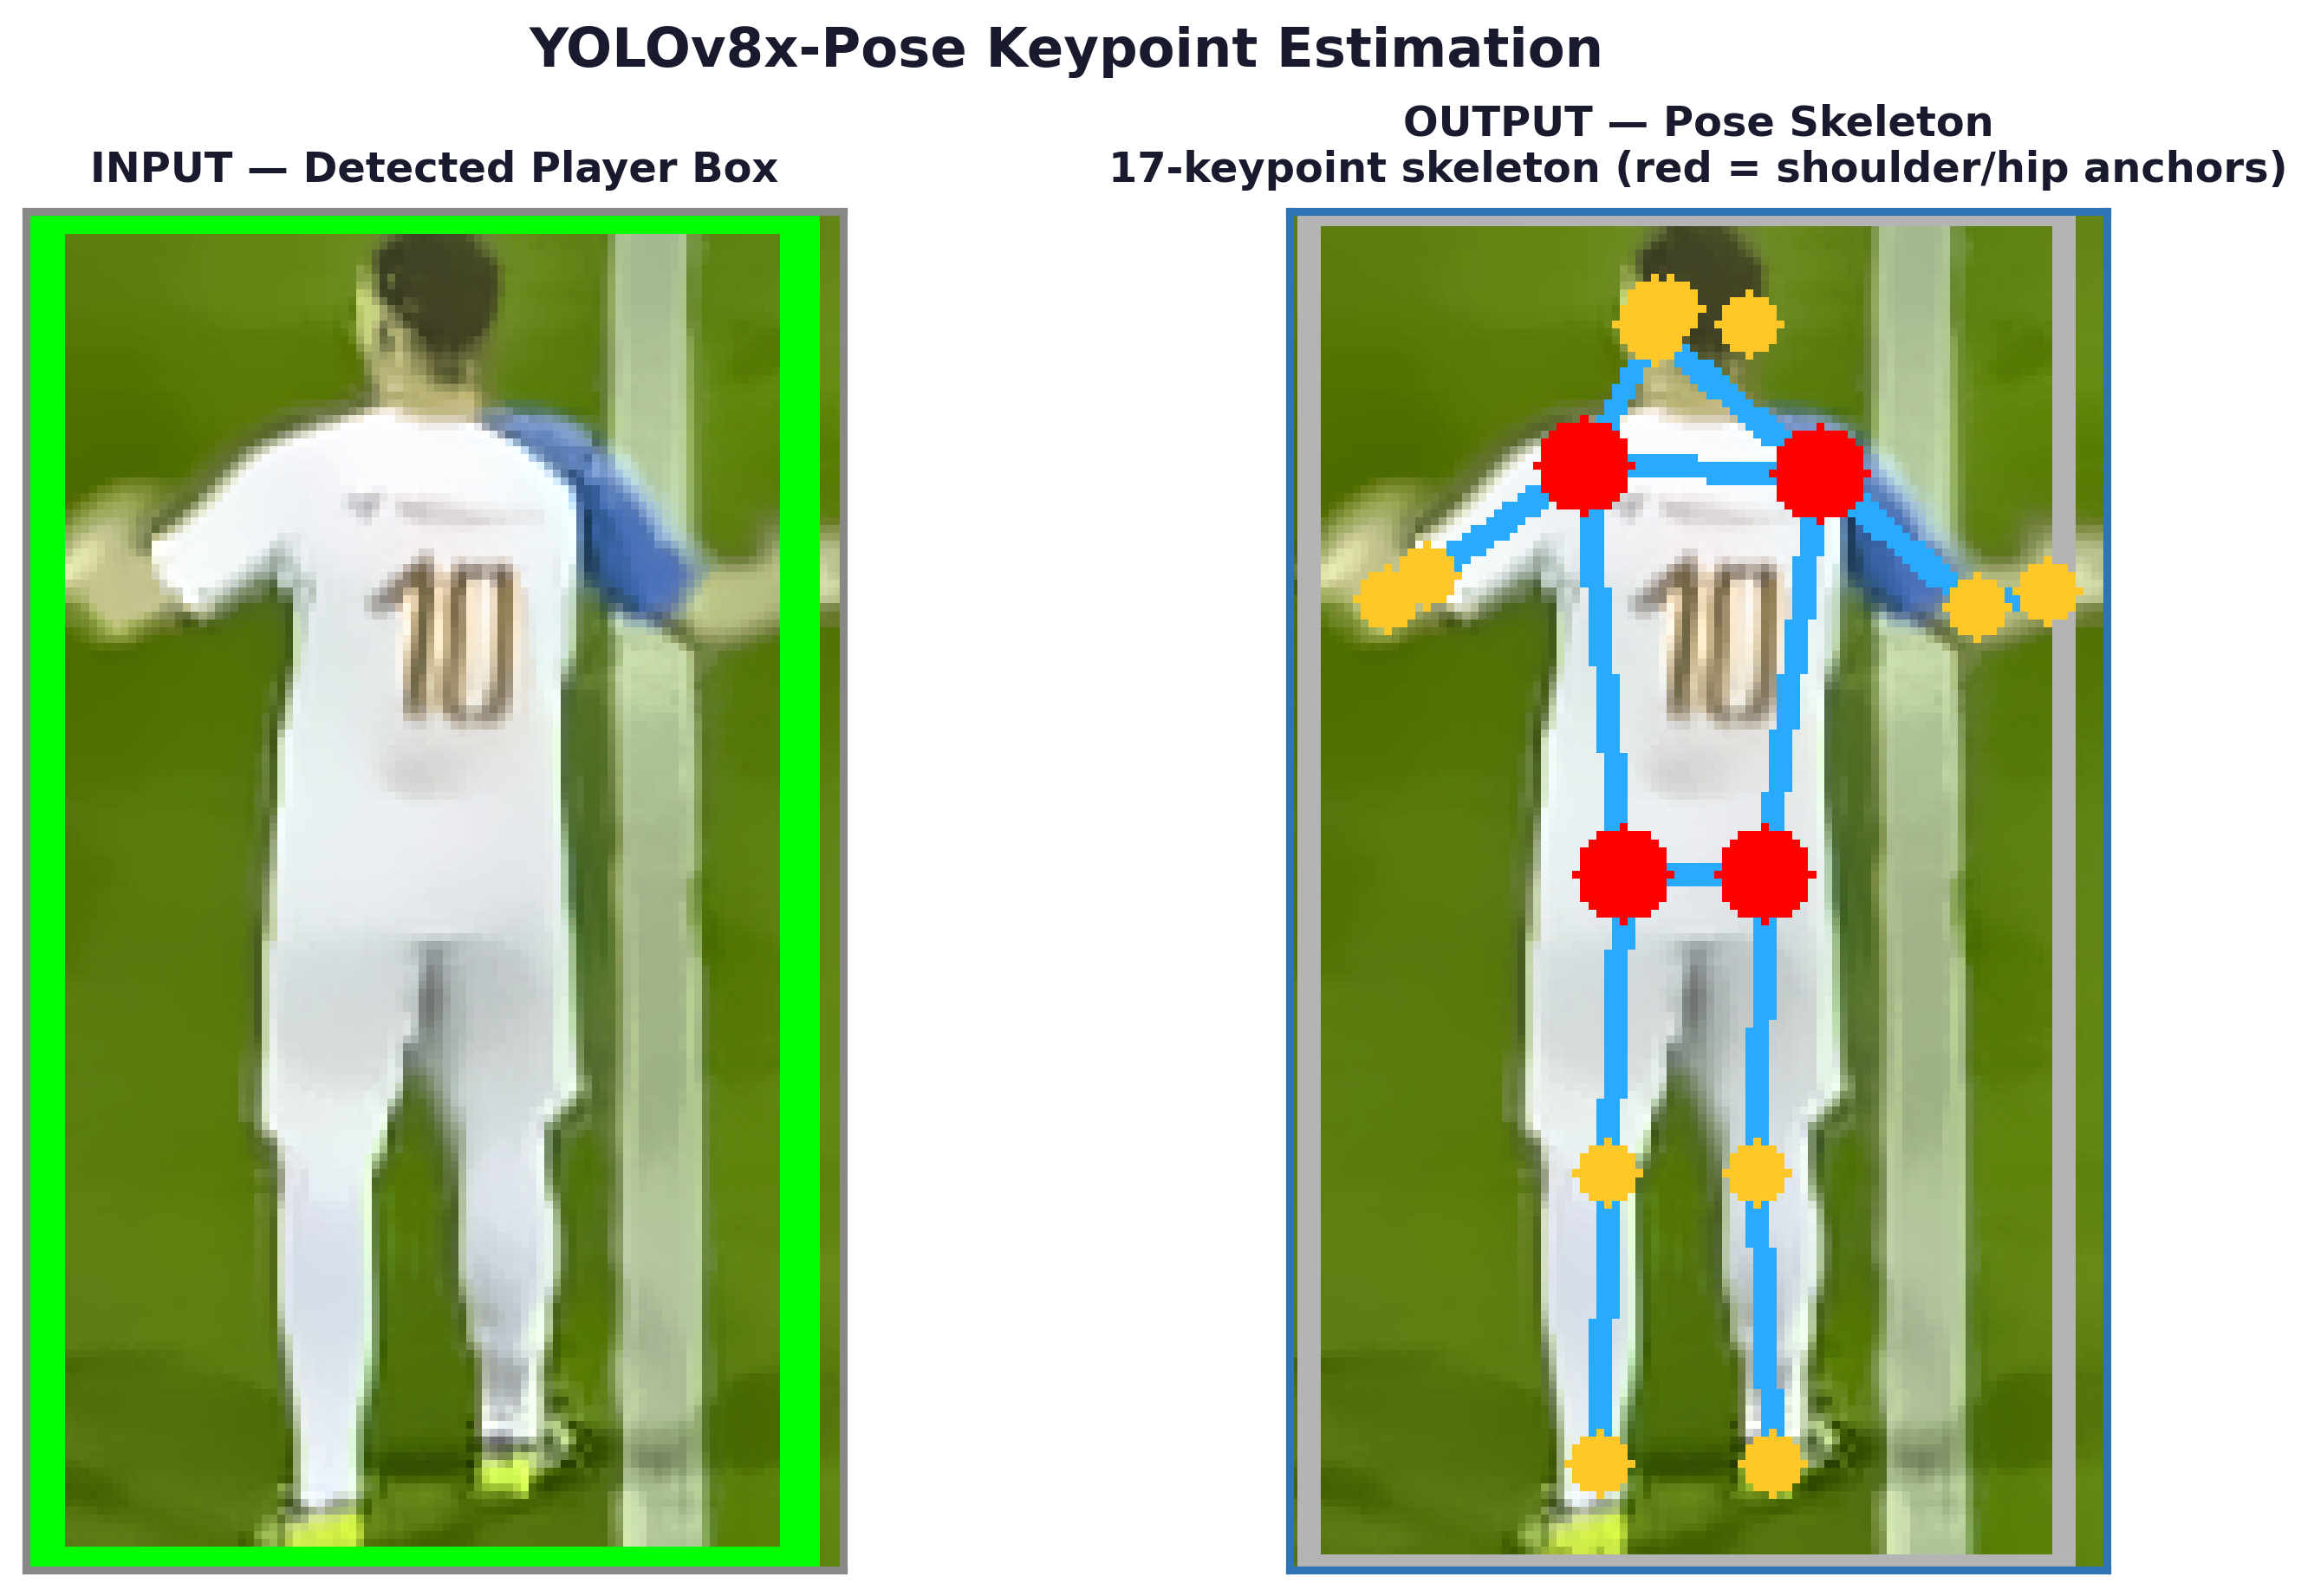
\includegraphics[width=0.85\textwidth]{figures/steps_image/fig_pose_estimation.png}
    \caption{YOLOv8x-Pose keypoint estimation (Section~\ref{sec:models}).
    The detected player box is passed to \texttt{PoseHelper}, which
    predicts a 17-keypoint skeleton; the shoulder and hip keypoints
    (highlighted) act as anchors for torso localization as formalized
    in Equation~\ref{eq:torso-box}.}
    \label{fig:step-img-pose}
\end{figure}

\begin{figure}[H]
    \centering
    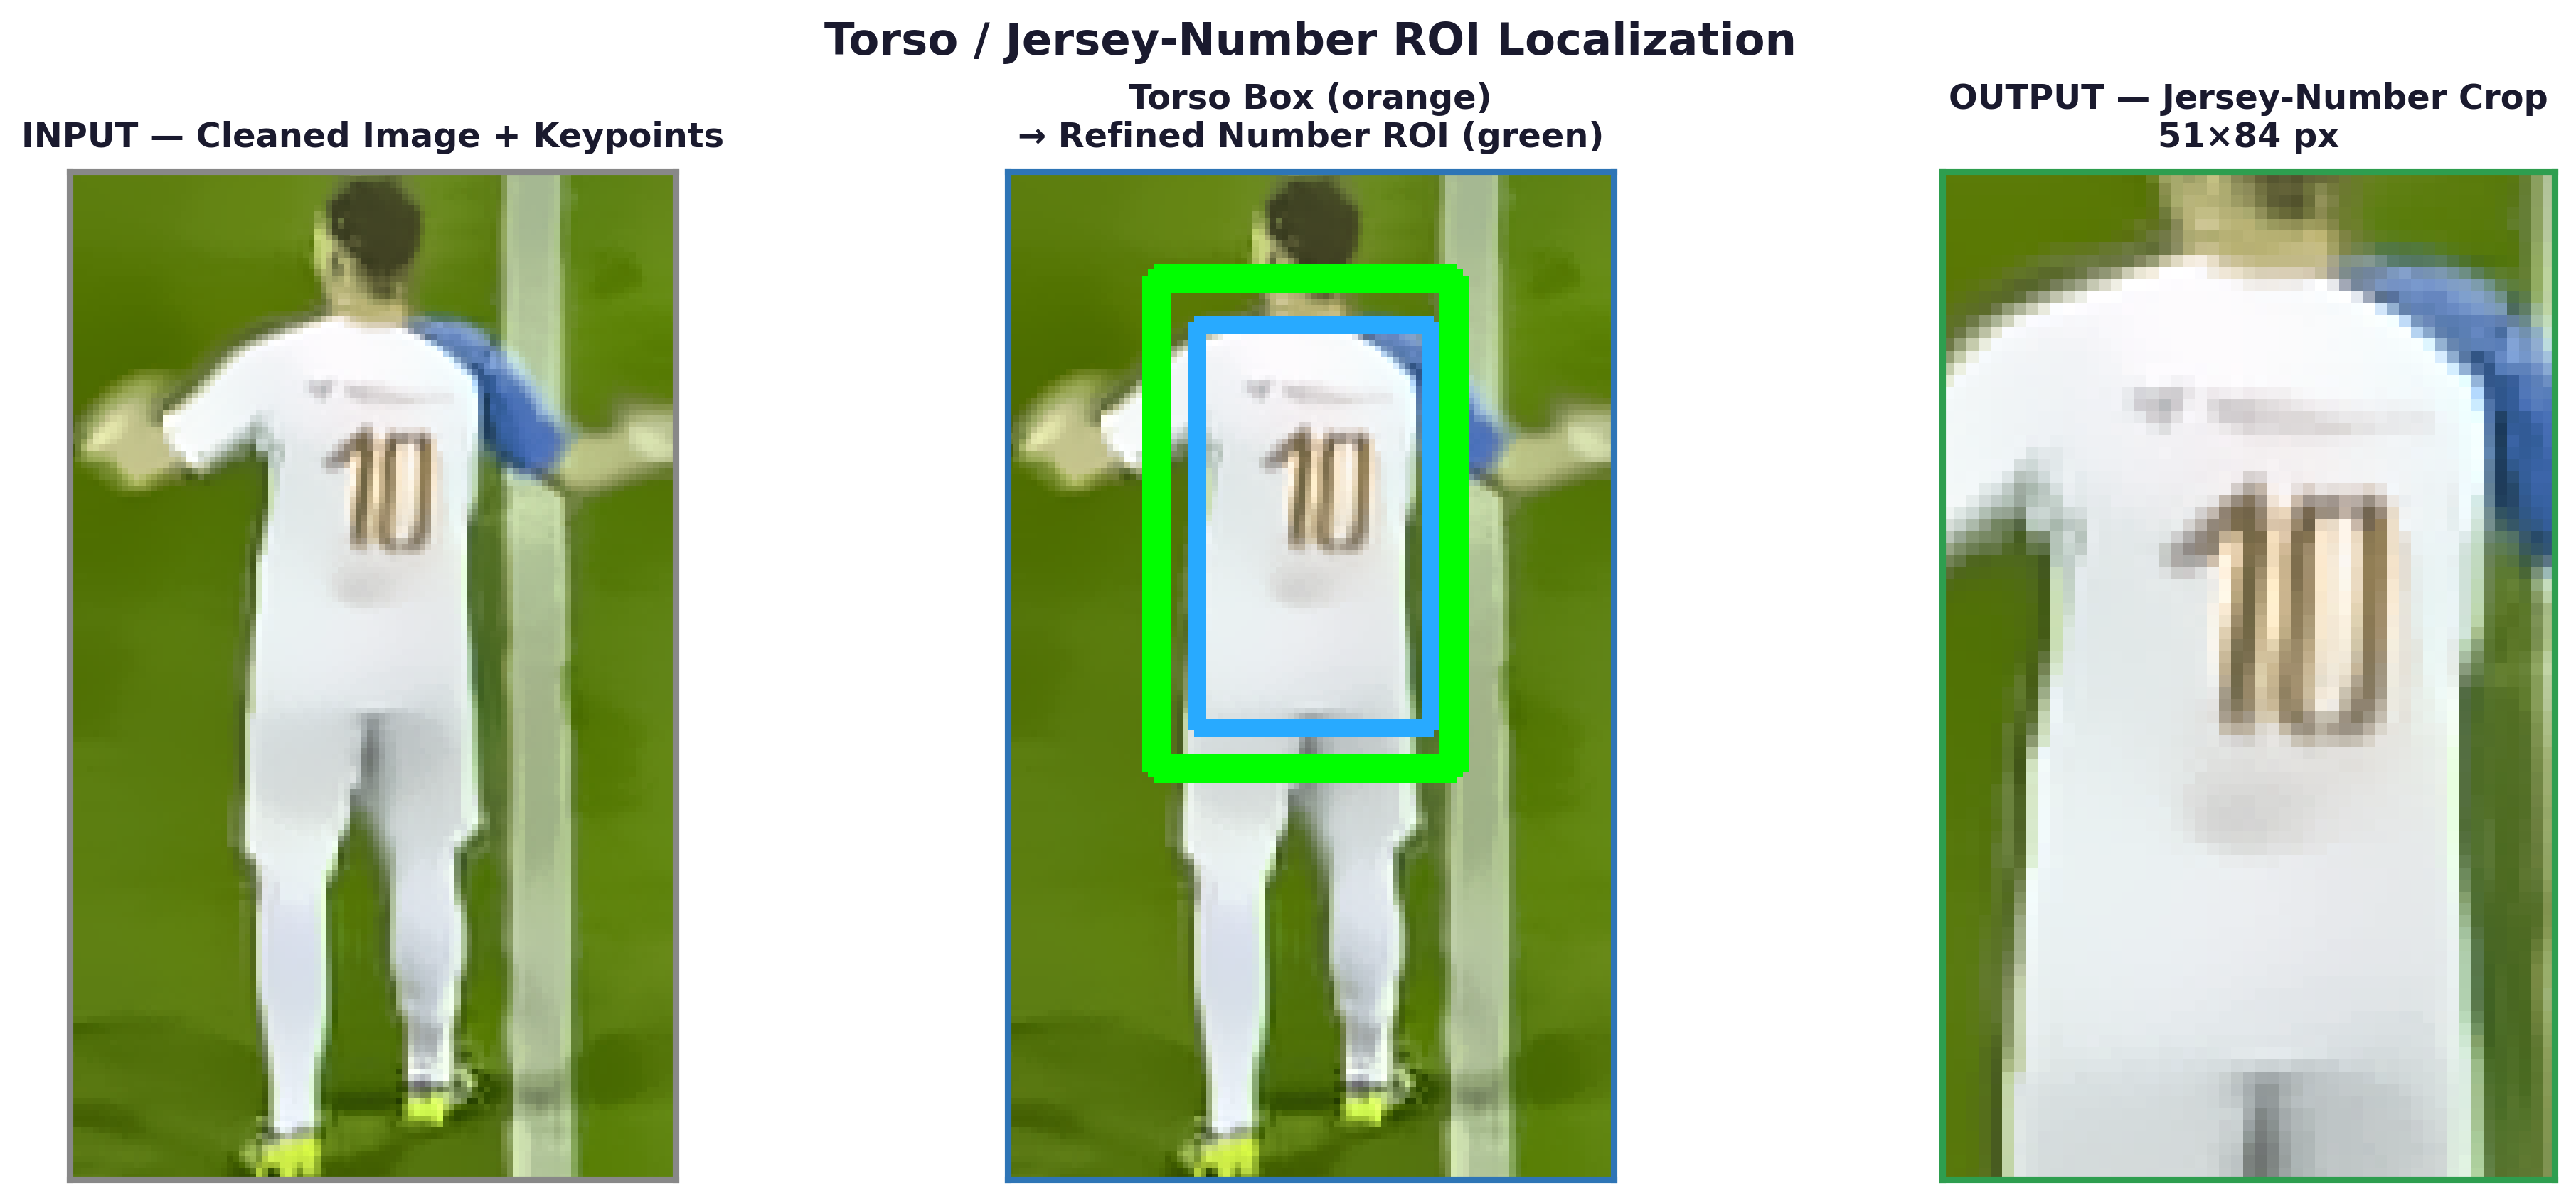
\includegraphics[width=0.85\textwidth]{figures/steps_image/fig_roi_localization.png}
    \caption{Torso and jersey-number ROI localization. The orange box
    shows the torso region derived from the pose keypoints via
    Equation~\ref{eq:torso-box}; the green box shows the refined
    jersey-number crop after applying the proportional margins from
    Table~\ref{tab:hp-detection}, here yielding a $51\times84$~px crop.}
    \label{fig:step-img-roi}
\end{figure}

\begin{figure}[H]
    \centering
    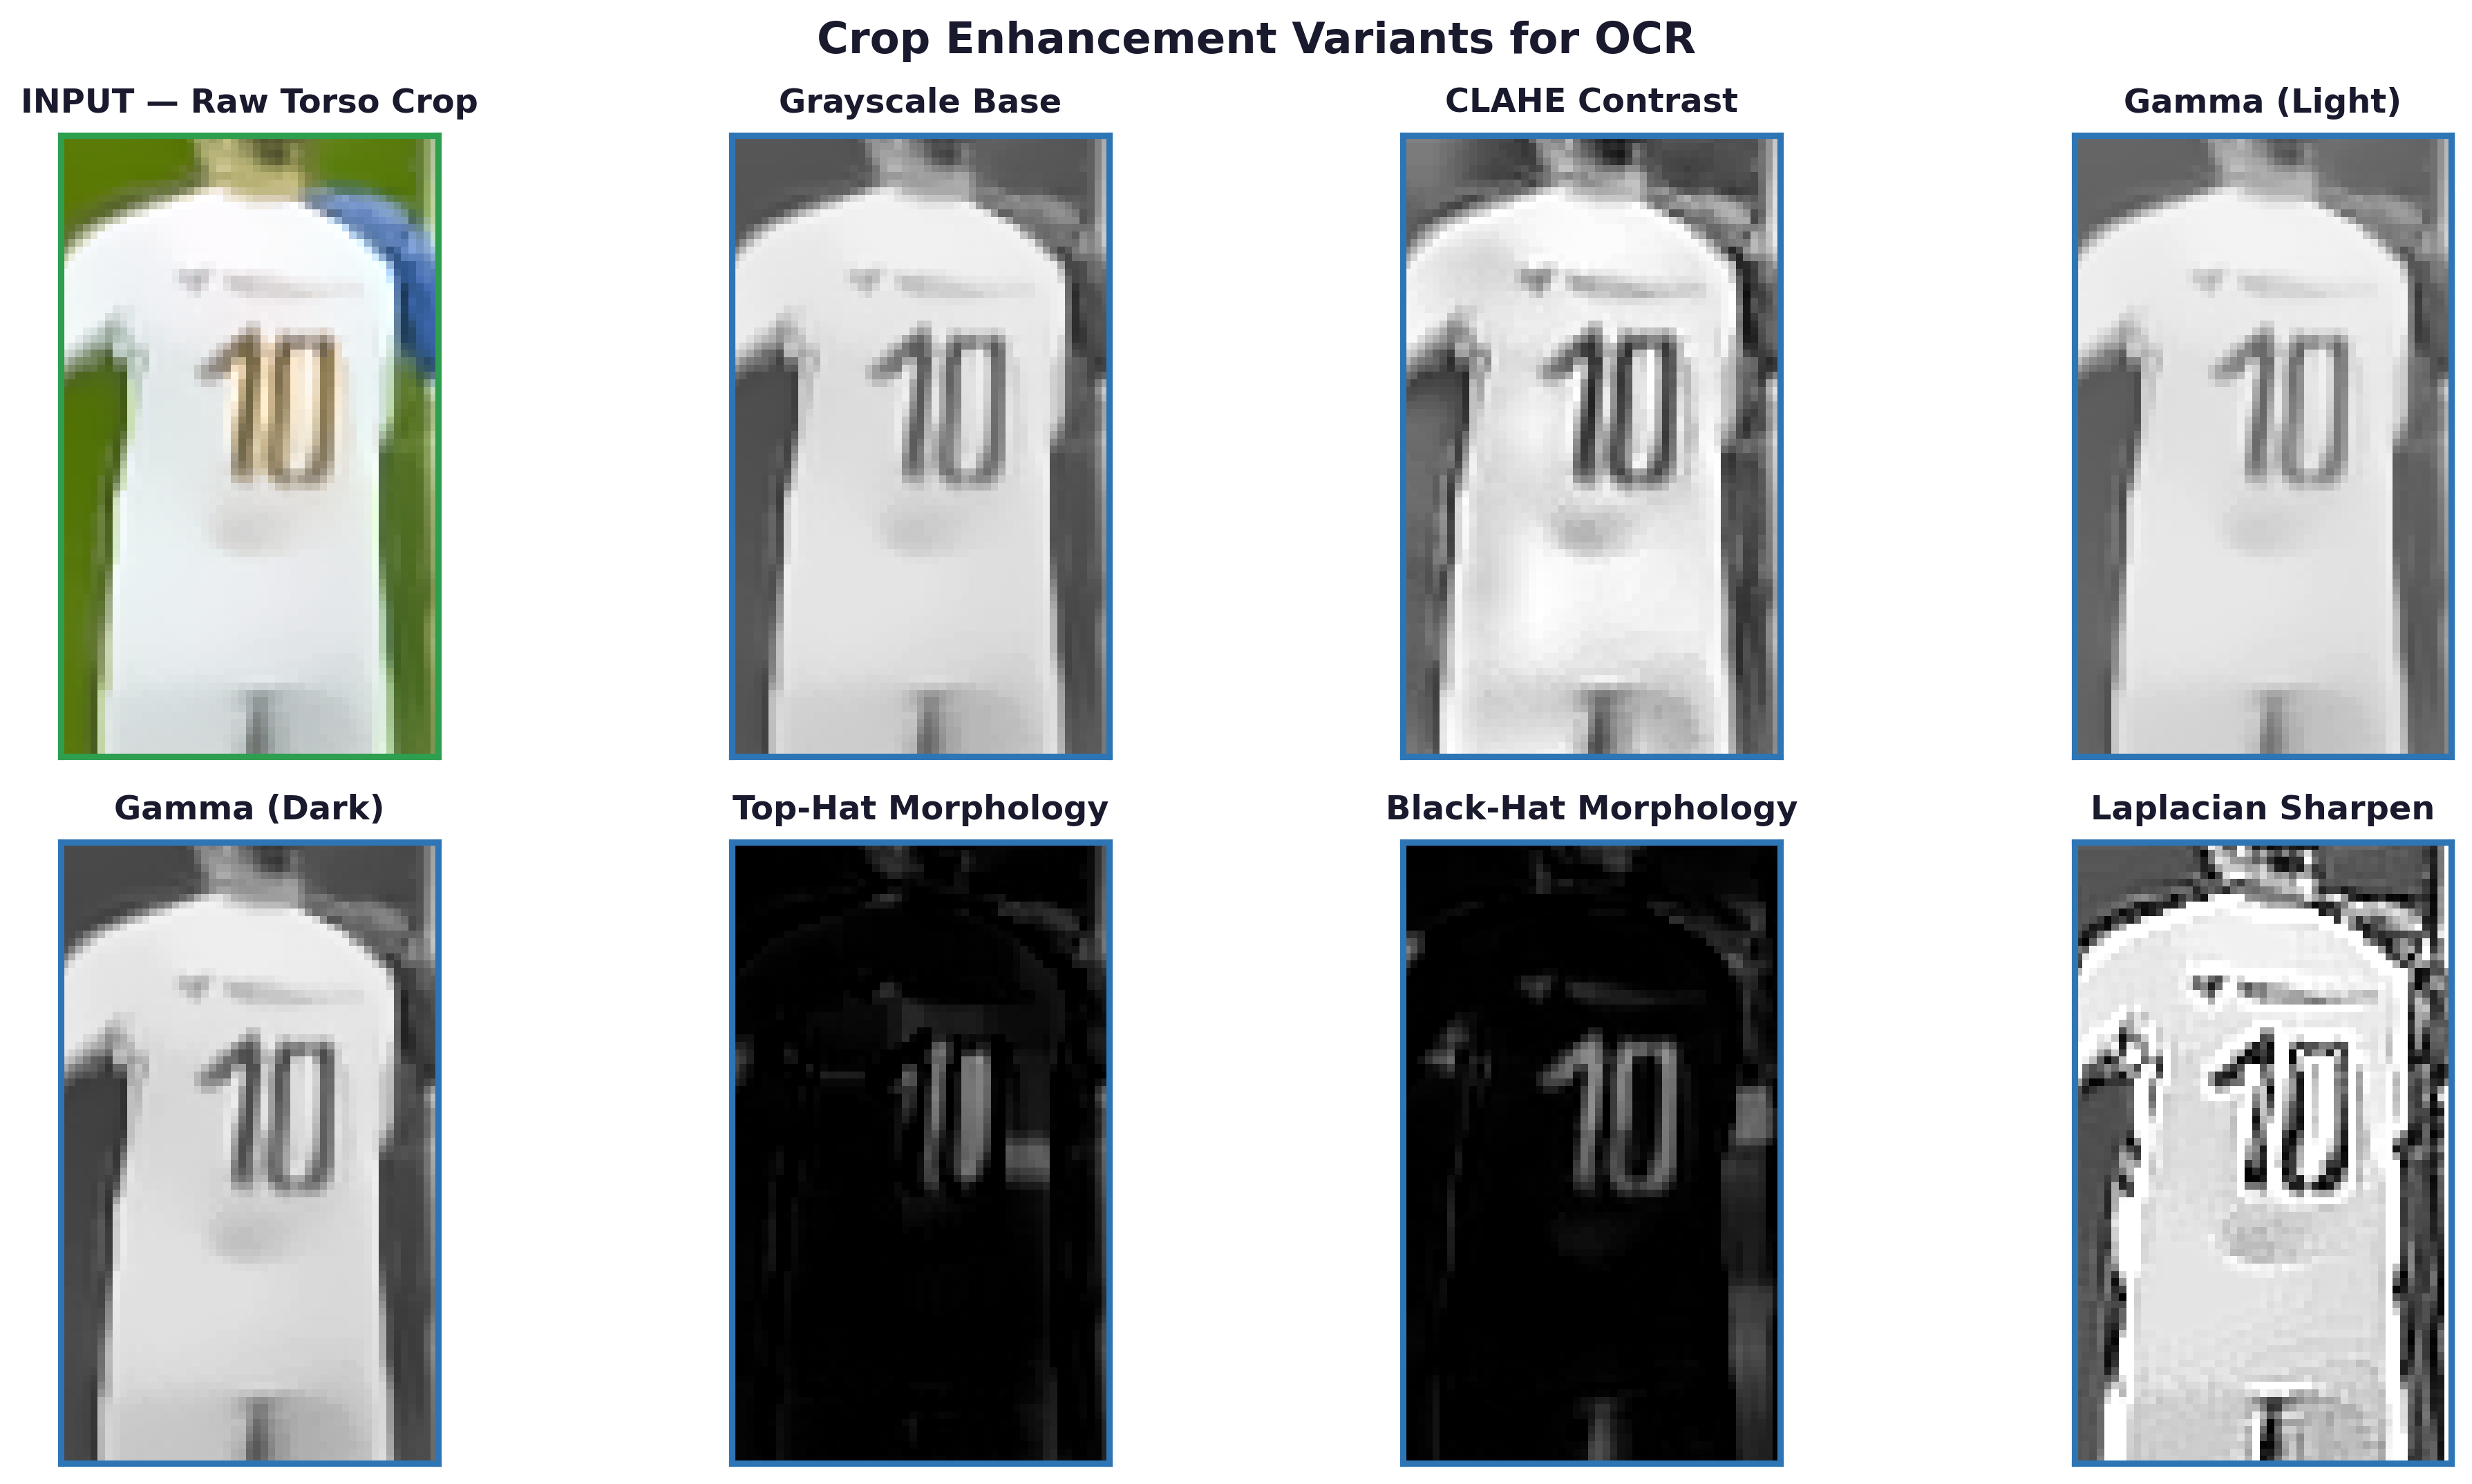
\includegraphics[width=0.85\textwidth]{figures/steps_image/fig_enhancement_variants.png}
    \caption{Crop-level enhancement variants (Section~\ref{sec:preprocessing}).
    From the raw torso crop, the pipeline generates multiple enhanced
    views --- grayscale base, CLAHE contrast, adaptive gamma (light and
    dark), top-hat and black-hat morphology, and Laplacian sharpening
    --- each of which is independently offered to the OCR stage.}
    \label{fig:step-img-enhance}
\end{figure}

\begin{figure}[H]
    \centering
    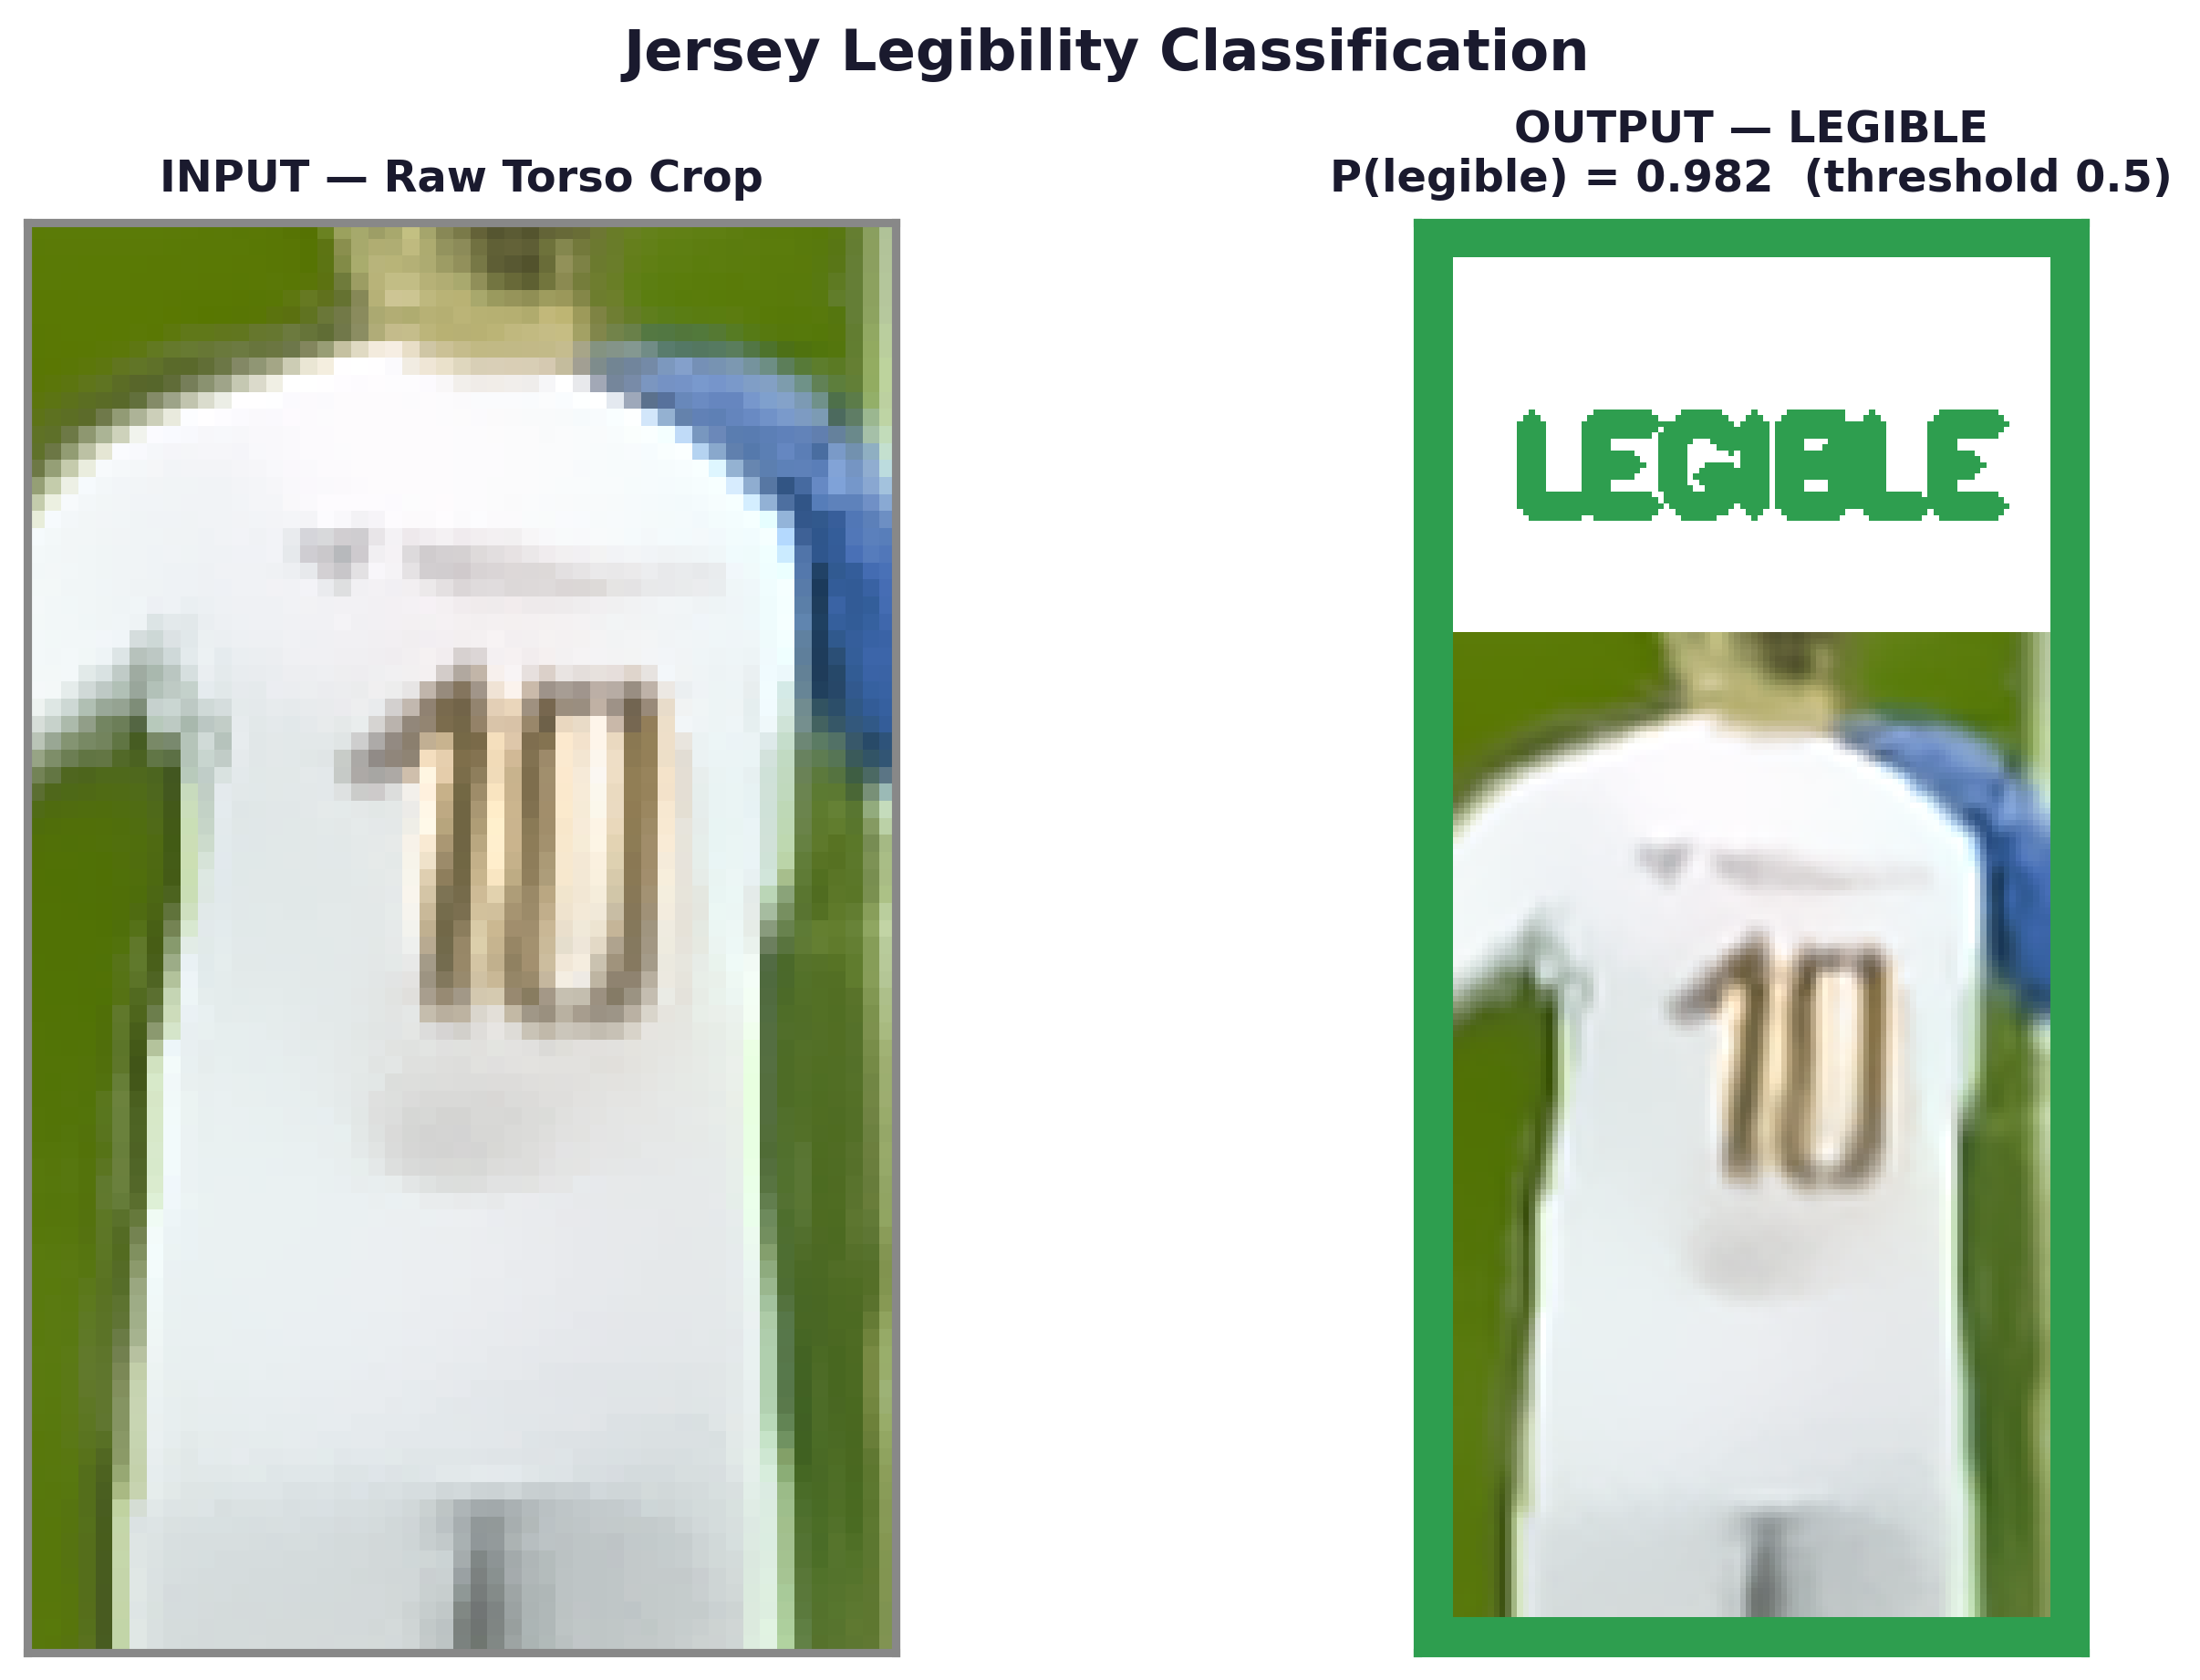
\includegraphics[width=0.75\textwidth]{figures/steps_image/fig_legibility.png}
    \caption{Legibility classification (Section~\ref{sec:models}). The
    raw torso crop is scored by the ResNet-18 \texttt{LegibilityModel};
    in this example the crop is classified as legible with $P(\text{legible})
    = 0.982$ against the 0.5 decision threshold.}
    \label{fig:step-img-legibility}
\end{figure}

\begin{figure}[H]
    \centering
    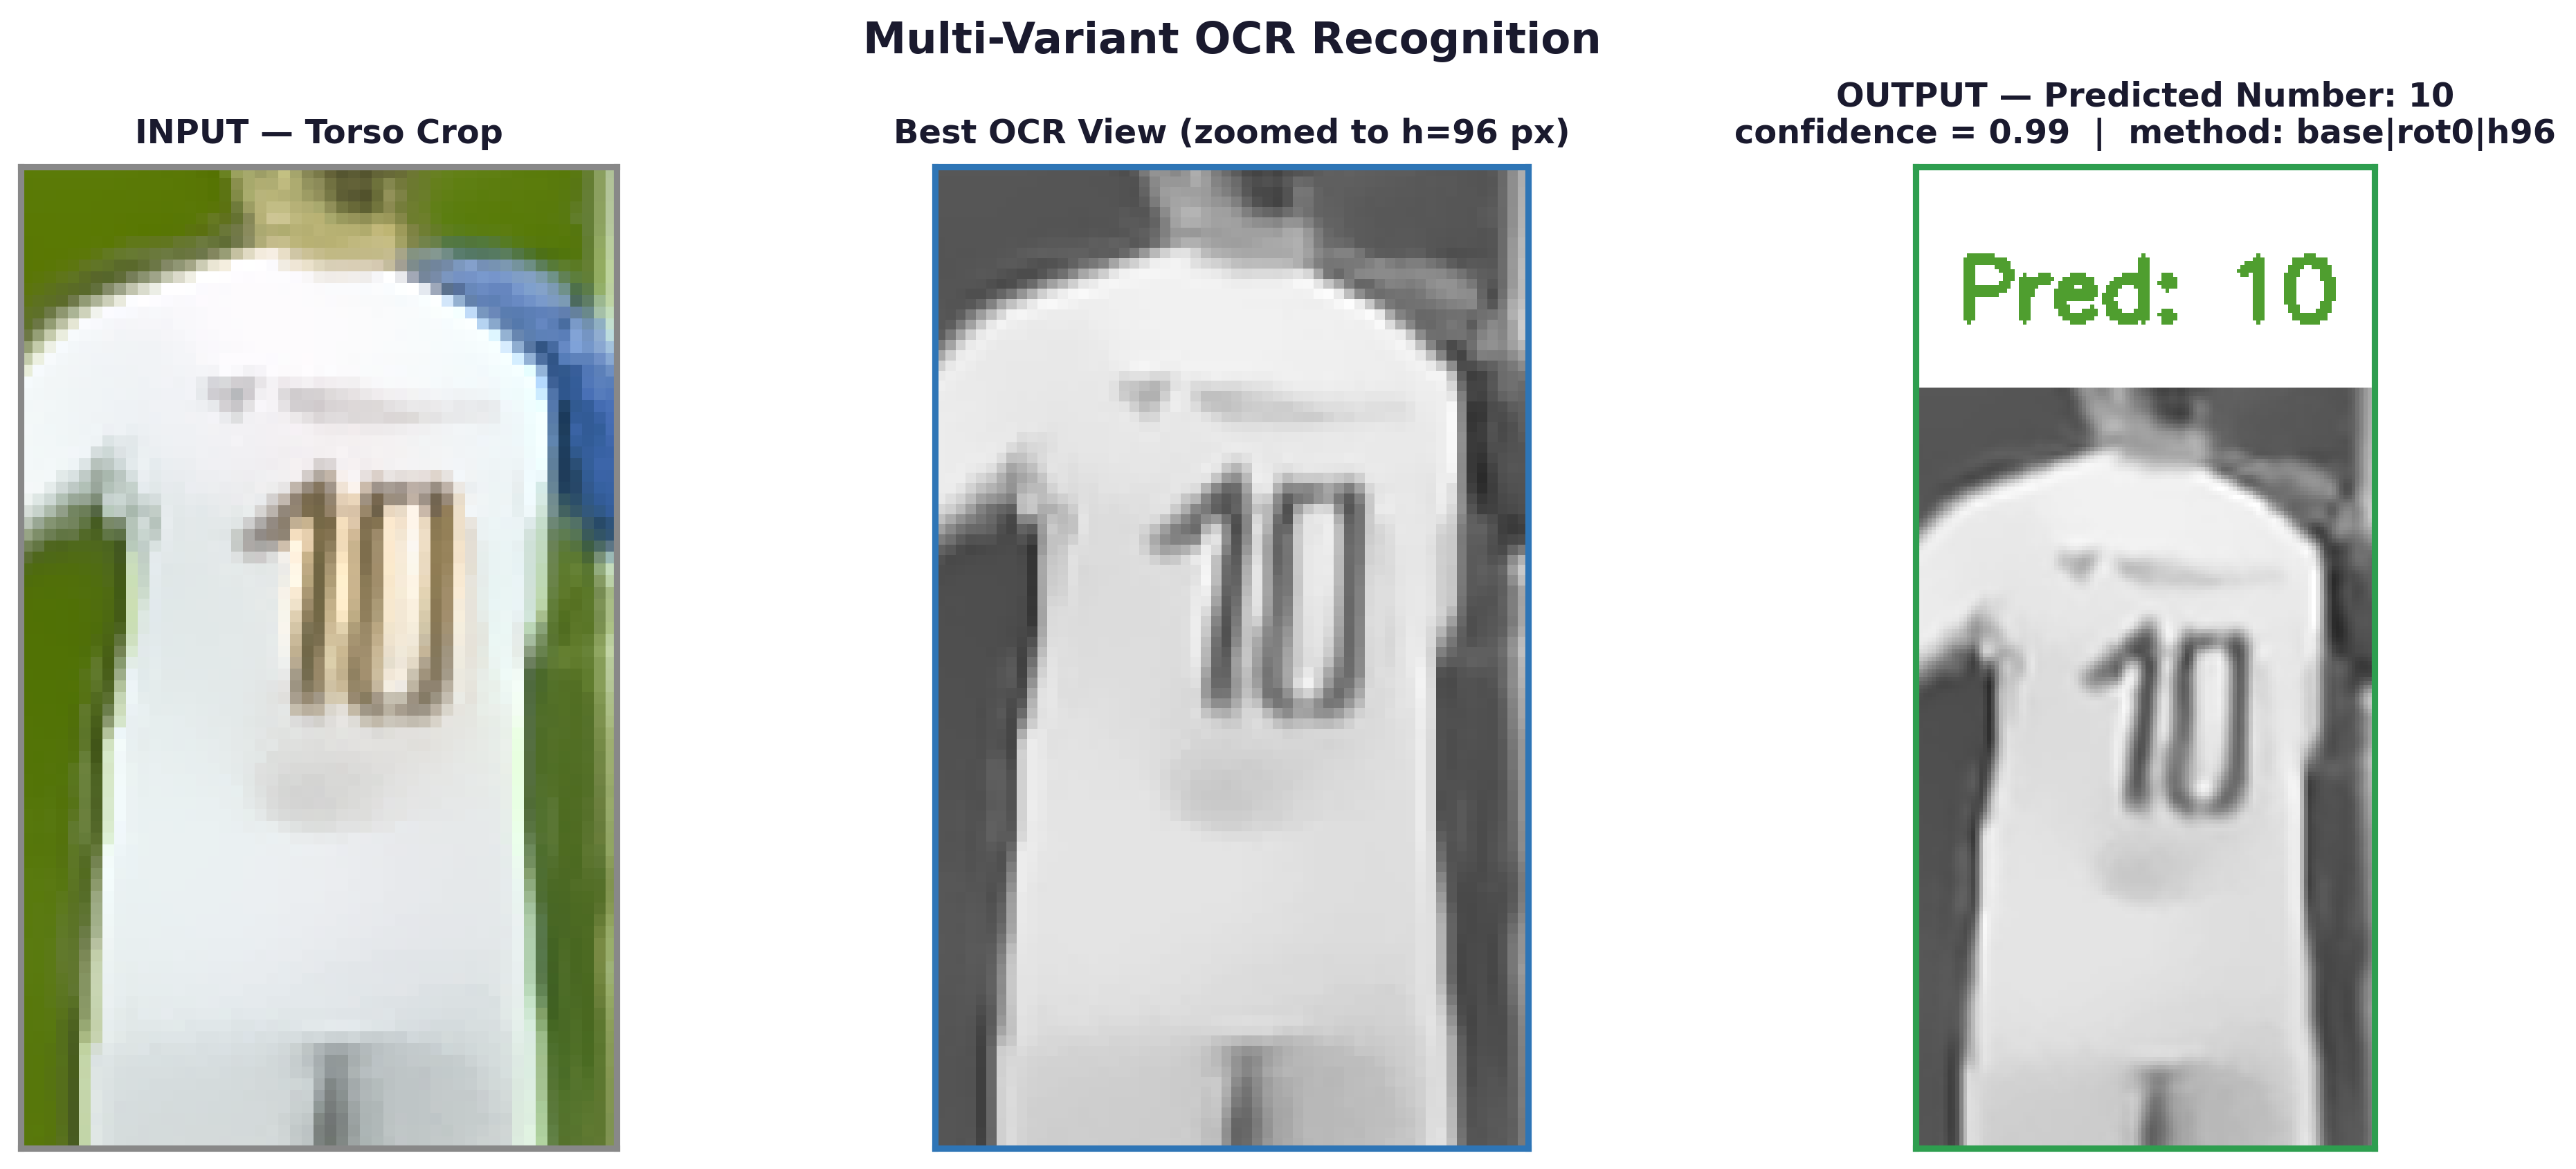
\includegraphics[width=0.85\textwidth]{figures/steps_image/fig_multivariant_ocr.png}
    \caption{Multi-variant OCR recognition (Section~\ref{sec:multi-variant-ocr}).
    The best-scoring enhancement variant (here, the crop zoomed to
    $h{=}96$~px) is selected by Equation~\ref{eq:ocr-score} and passed
    to EasyOCR, producing the final predicted jersey number together
    with its confidence and the identifying method tag.}
    \label{fig:step-img-ocr}
\end{figure}

\section{Visual Process Walkthrough --- Video Pipeline}
\label{sec:video-visual-walkthrough}

This section presents the corresponding visual walkthrough for the
video pipeline, tracing one player track (track ID 1242 in clip
008.mp4) through every processing stage from raw detection to
ground-truth evaluation.

\begin{figure}[H]
    \centering
    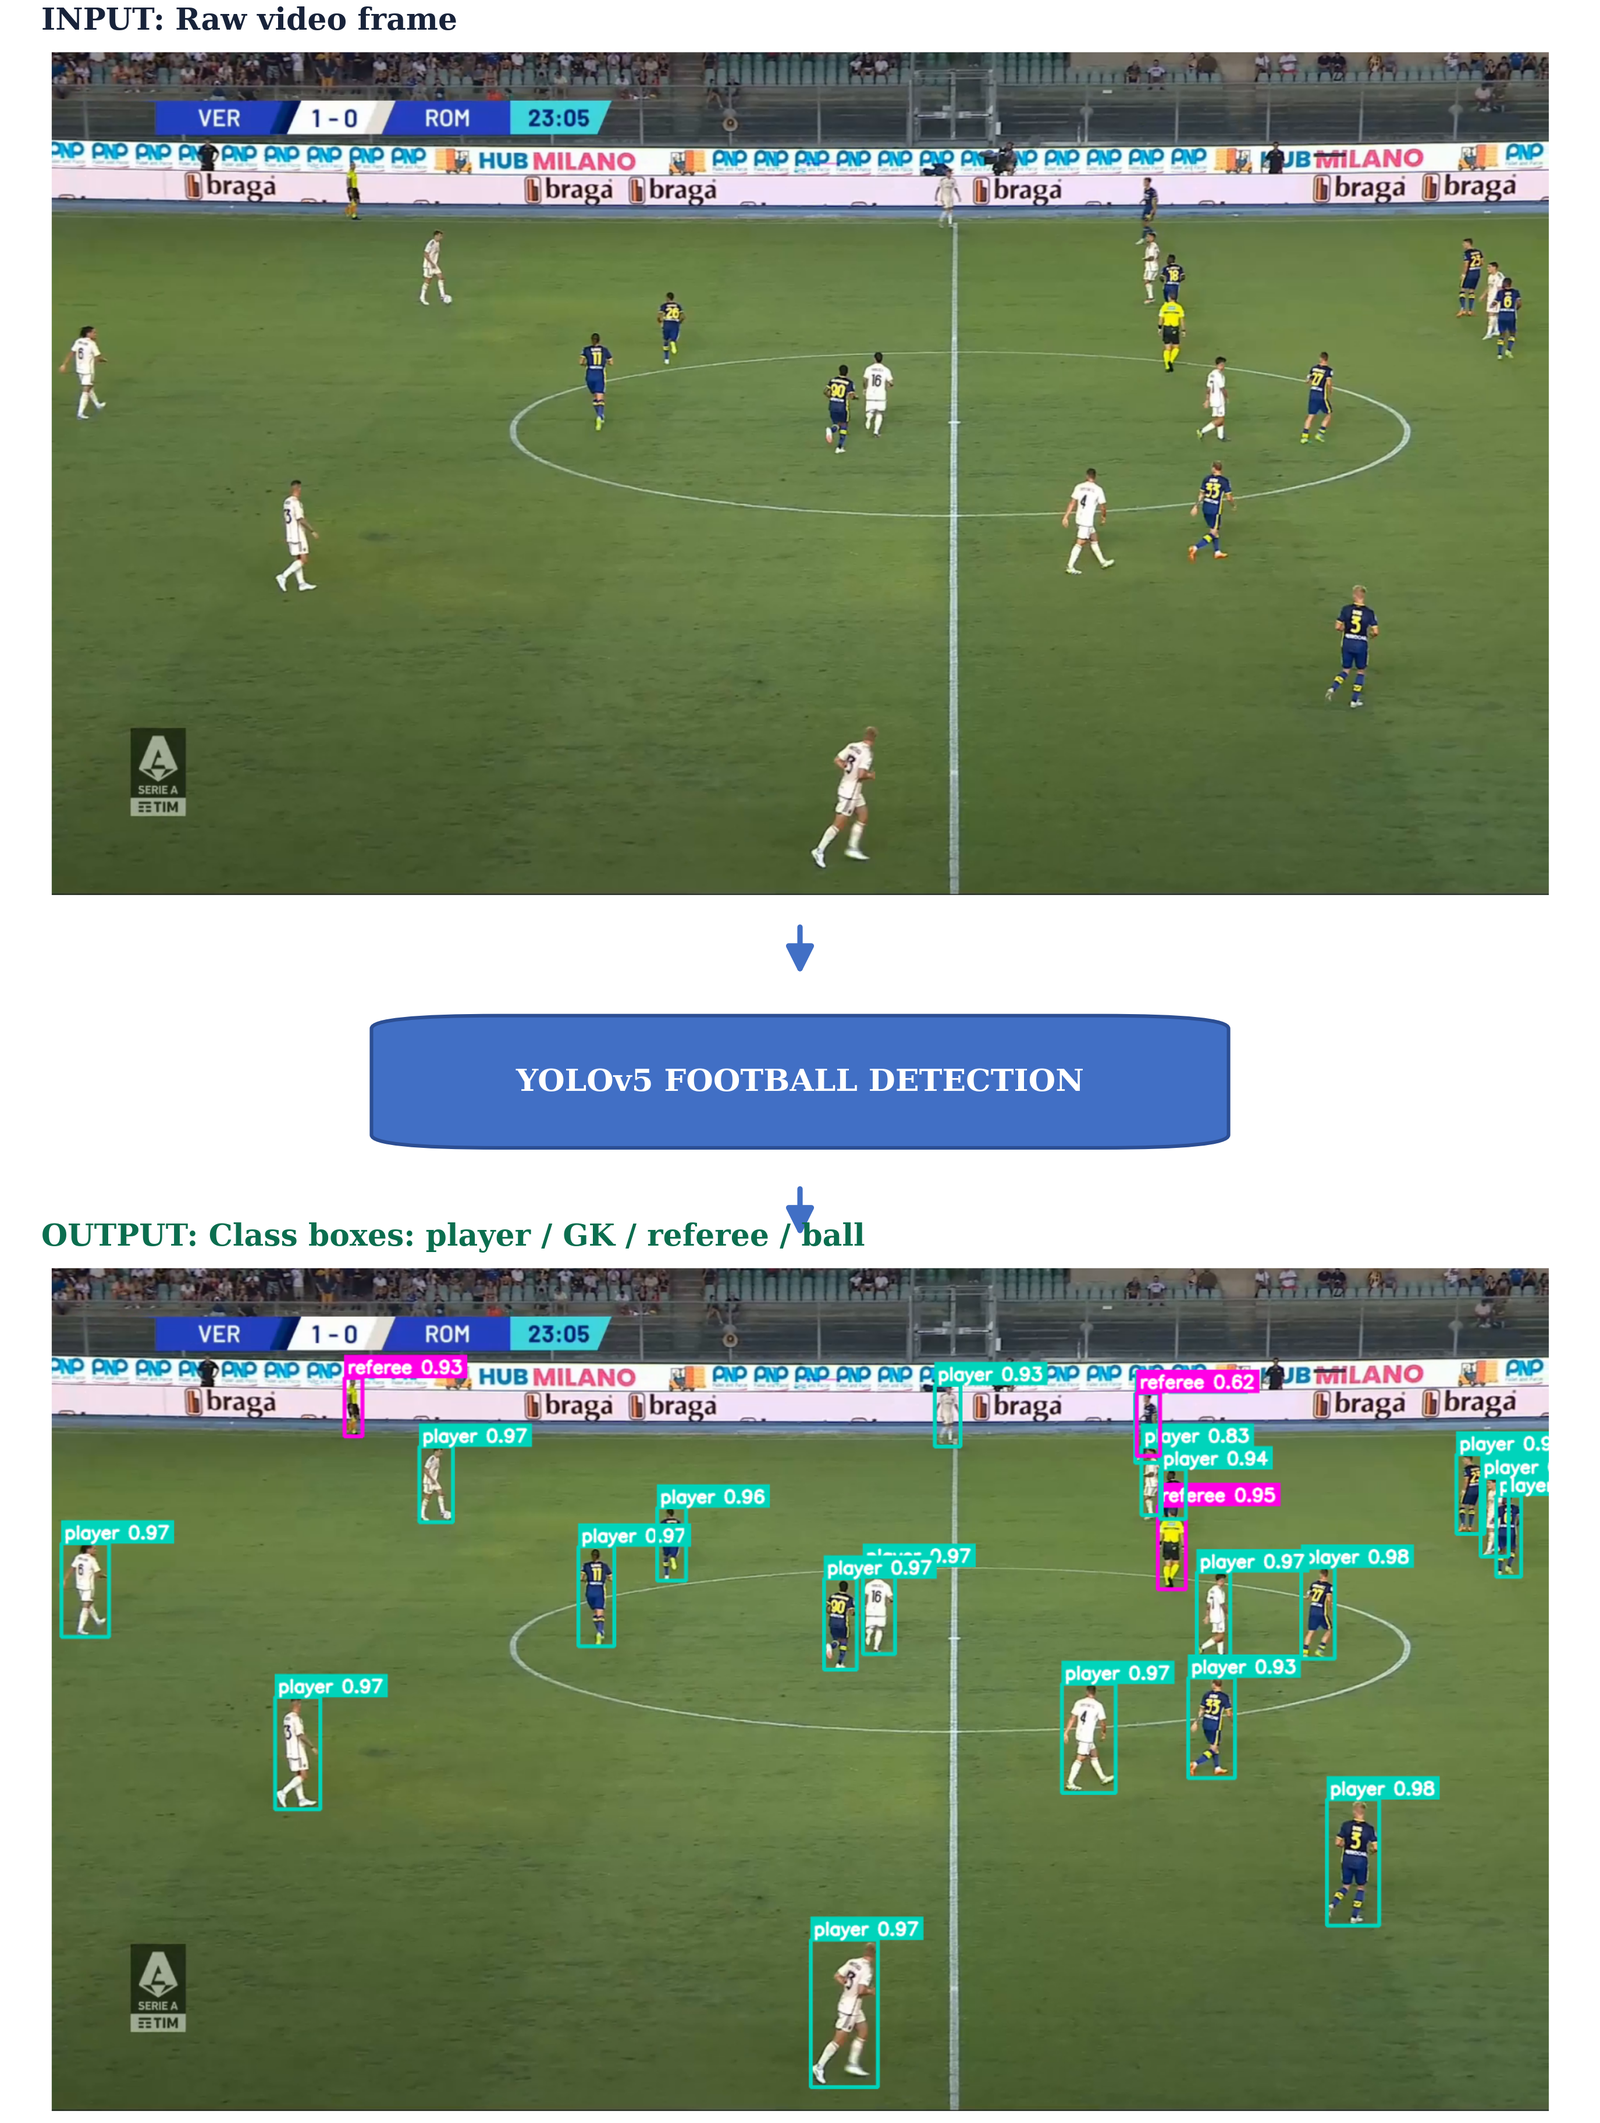
\includegraphics[width=1\textwidth]{figures/steps_video/step_1_figure.png}
    \caption{YOLOv5 football detection (Section~\ref{sec:models}). Each
    raw broadcast frame is passed through the football-specific YOLOv5
    model, producing per-player bounding boxes with class confidences
    (typically 0.93--0.98 for clearly visible players).}
    \label{fig:video-step1-detection}
\end{figure}

\begin{figure}[H]
    \centering
    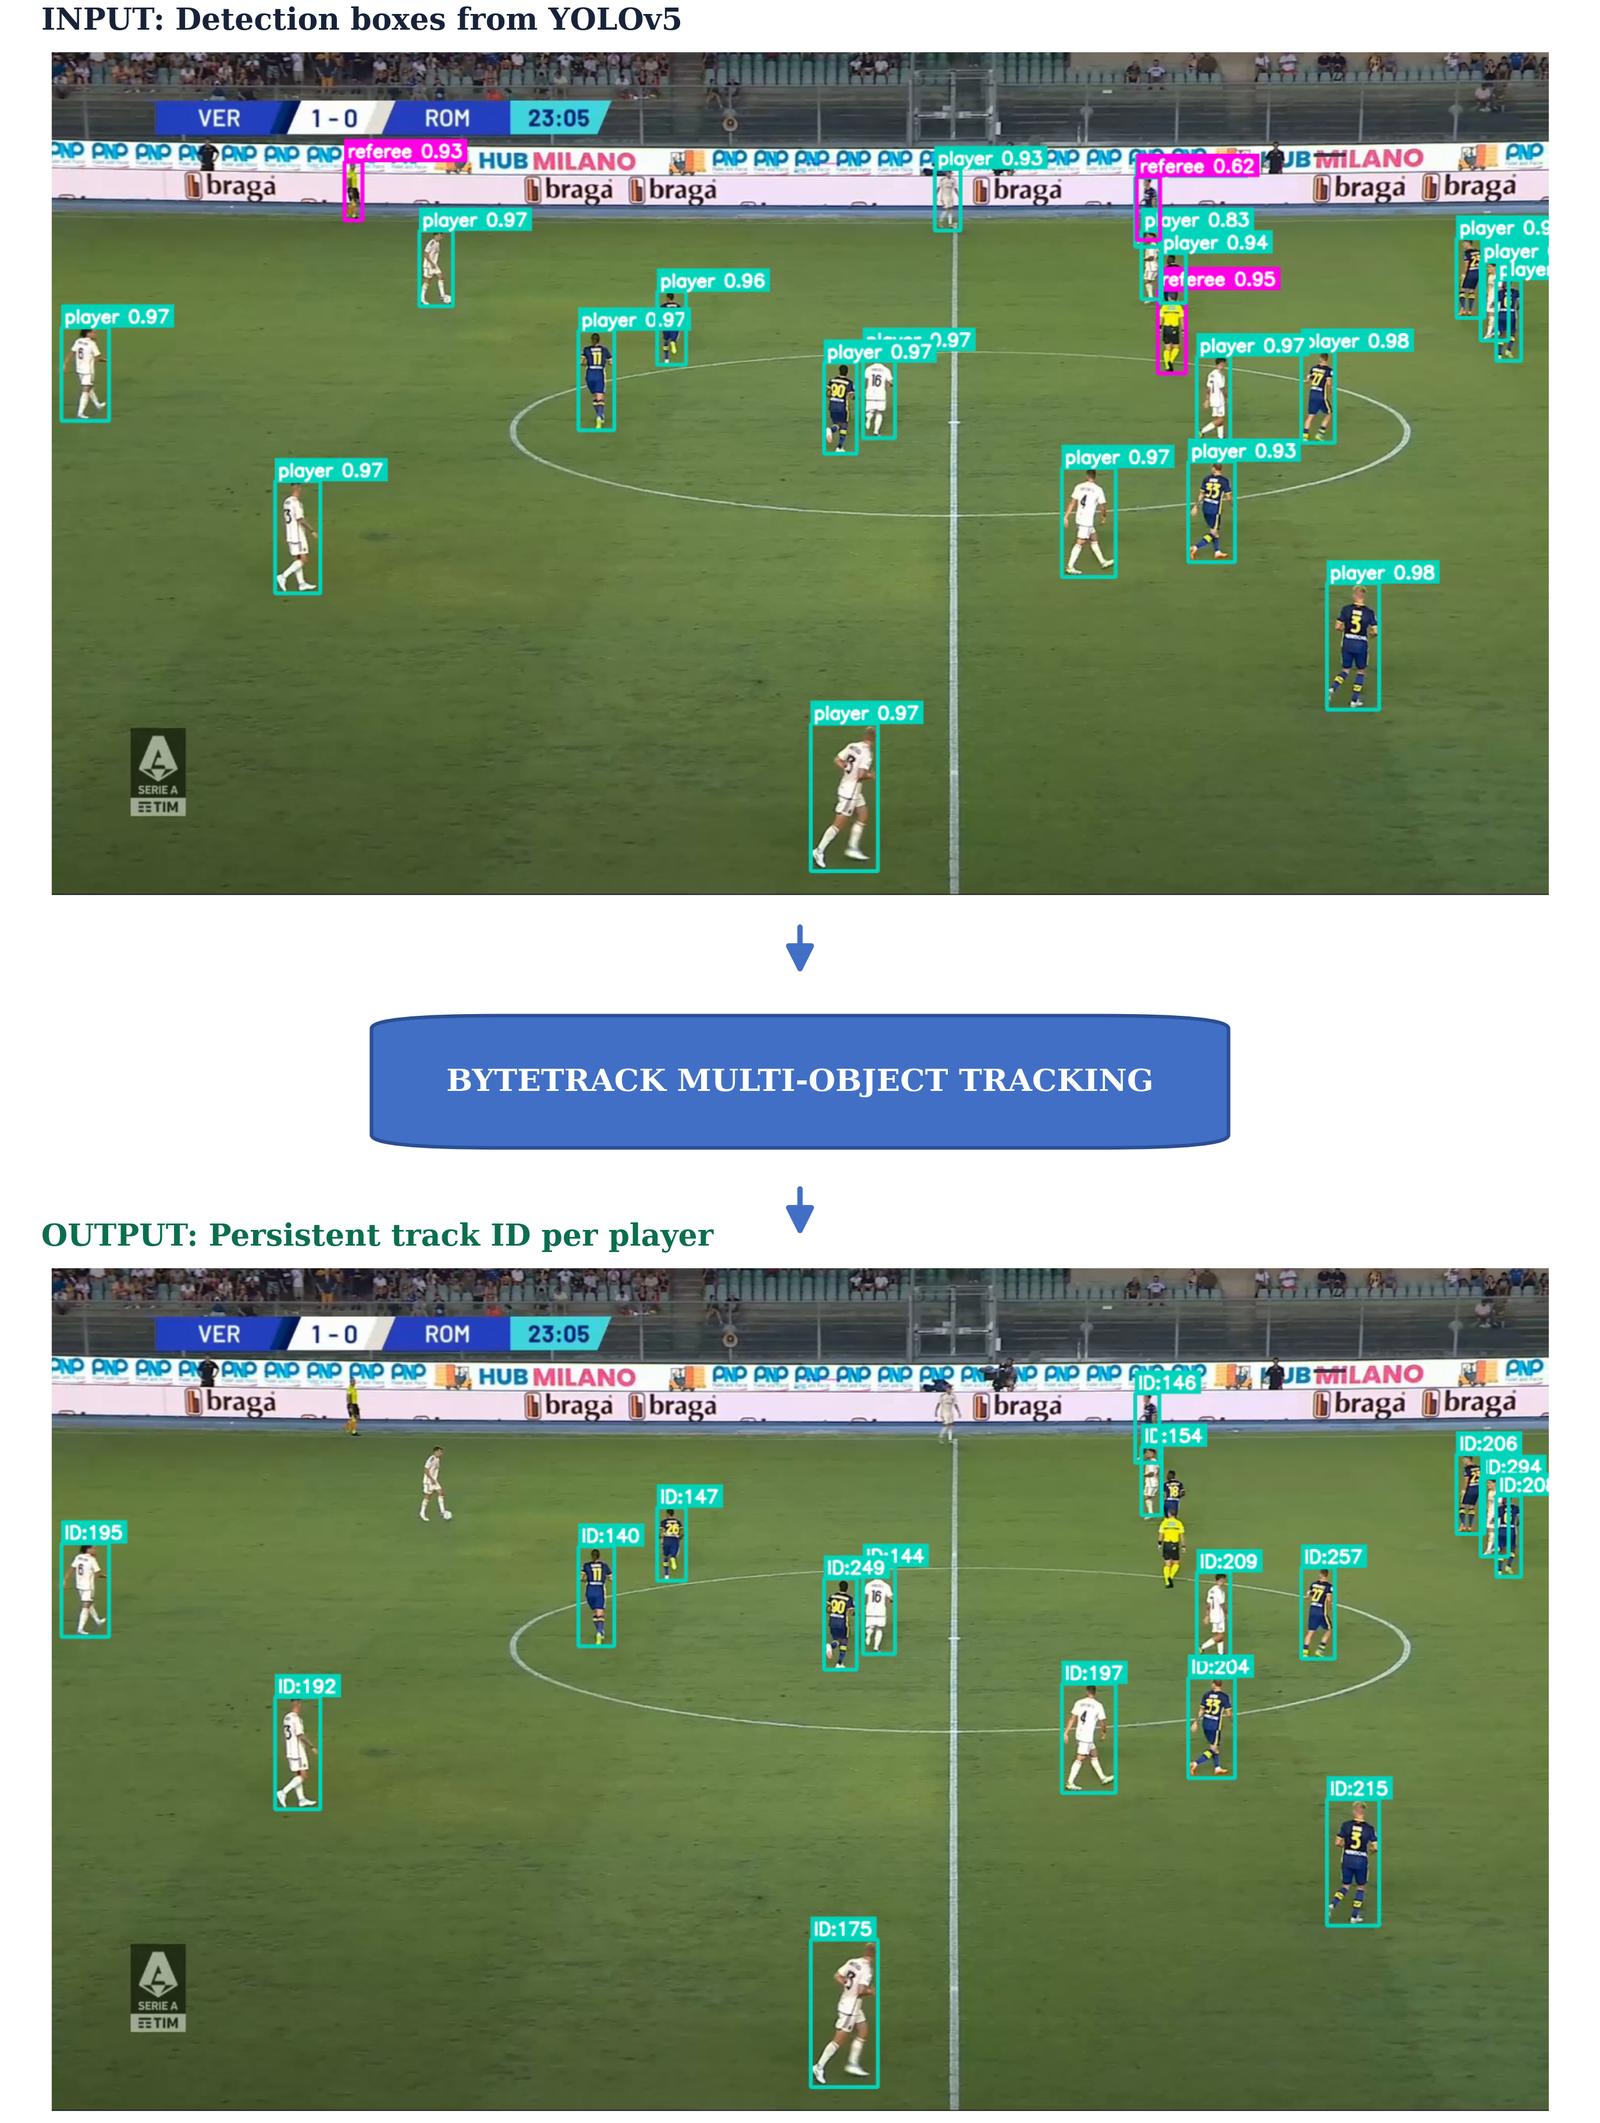
\includegraphics[width=1\textwidth]{figures/steps_video/step_2_figure.png}
    \caption{ByteTrack multi-object tracking (Section~\ref{sec:models}).
    Detection boxes from Figure~\ref{fig:video-step1-detection} are
    associated across frames via Equation~\ref{eq:bytetrack-cost},
    producing a persistent track ID for each player (e.g.\ ID:206,
    ID:154, ID:294, ID:20 in this frame).}
    \label{fig:video-step2-tracking}
\end{figure}

\begin{figure}[H]
    \centering
    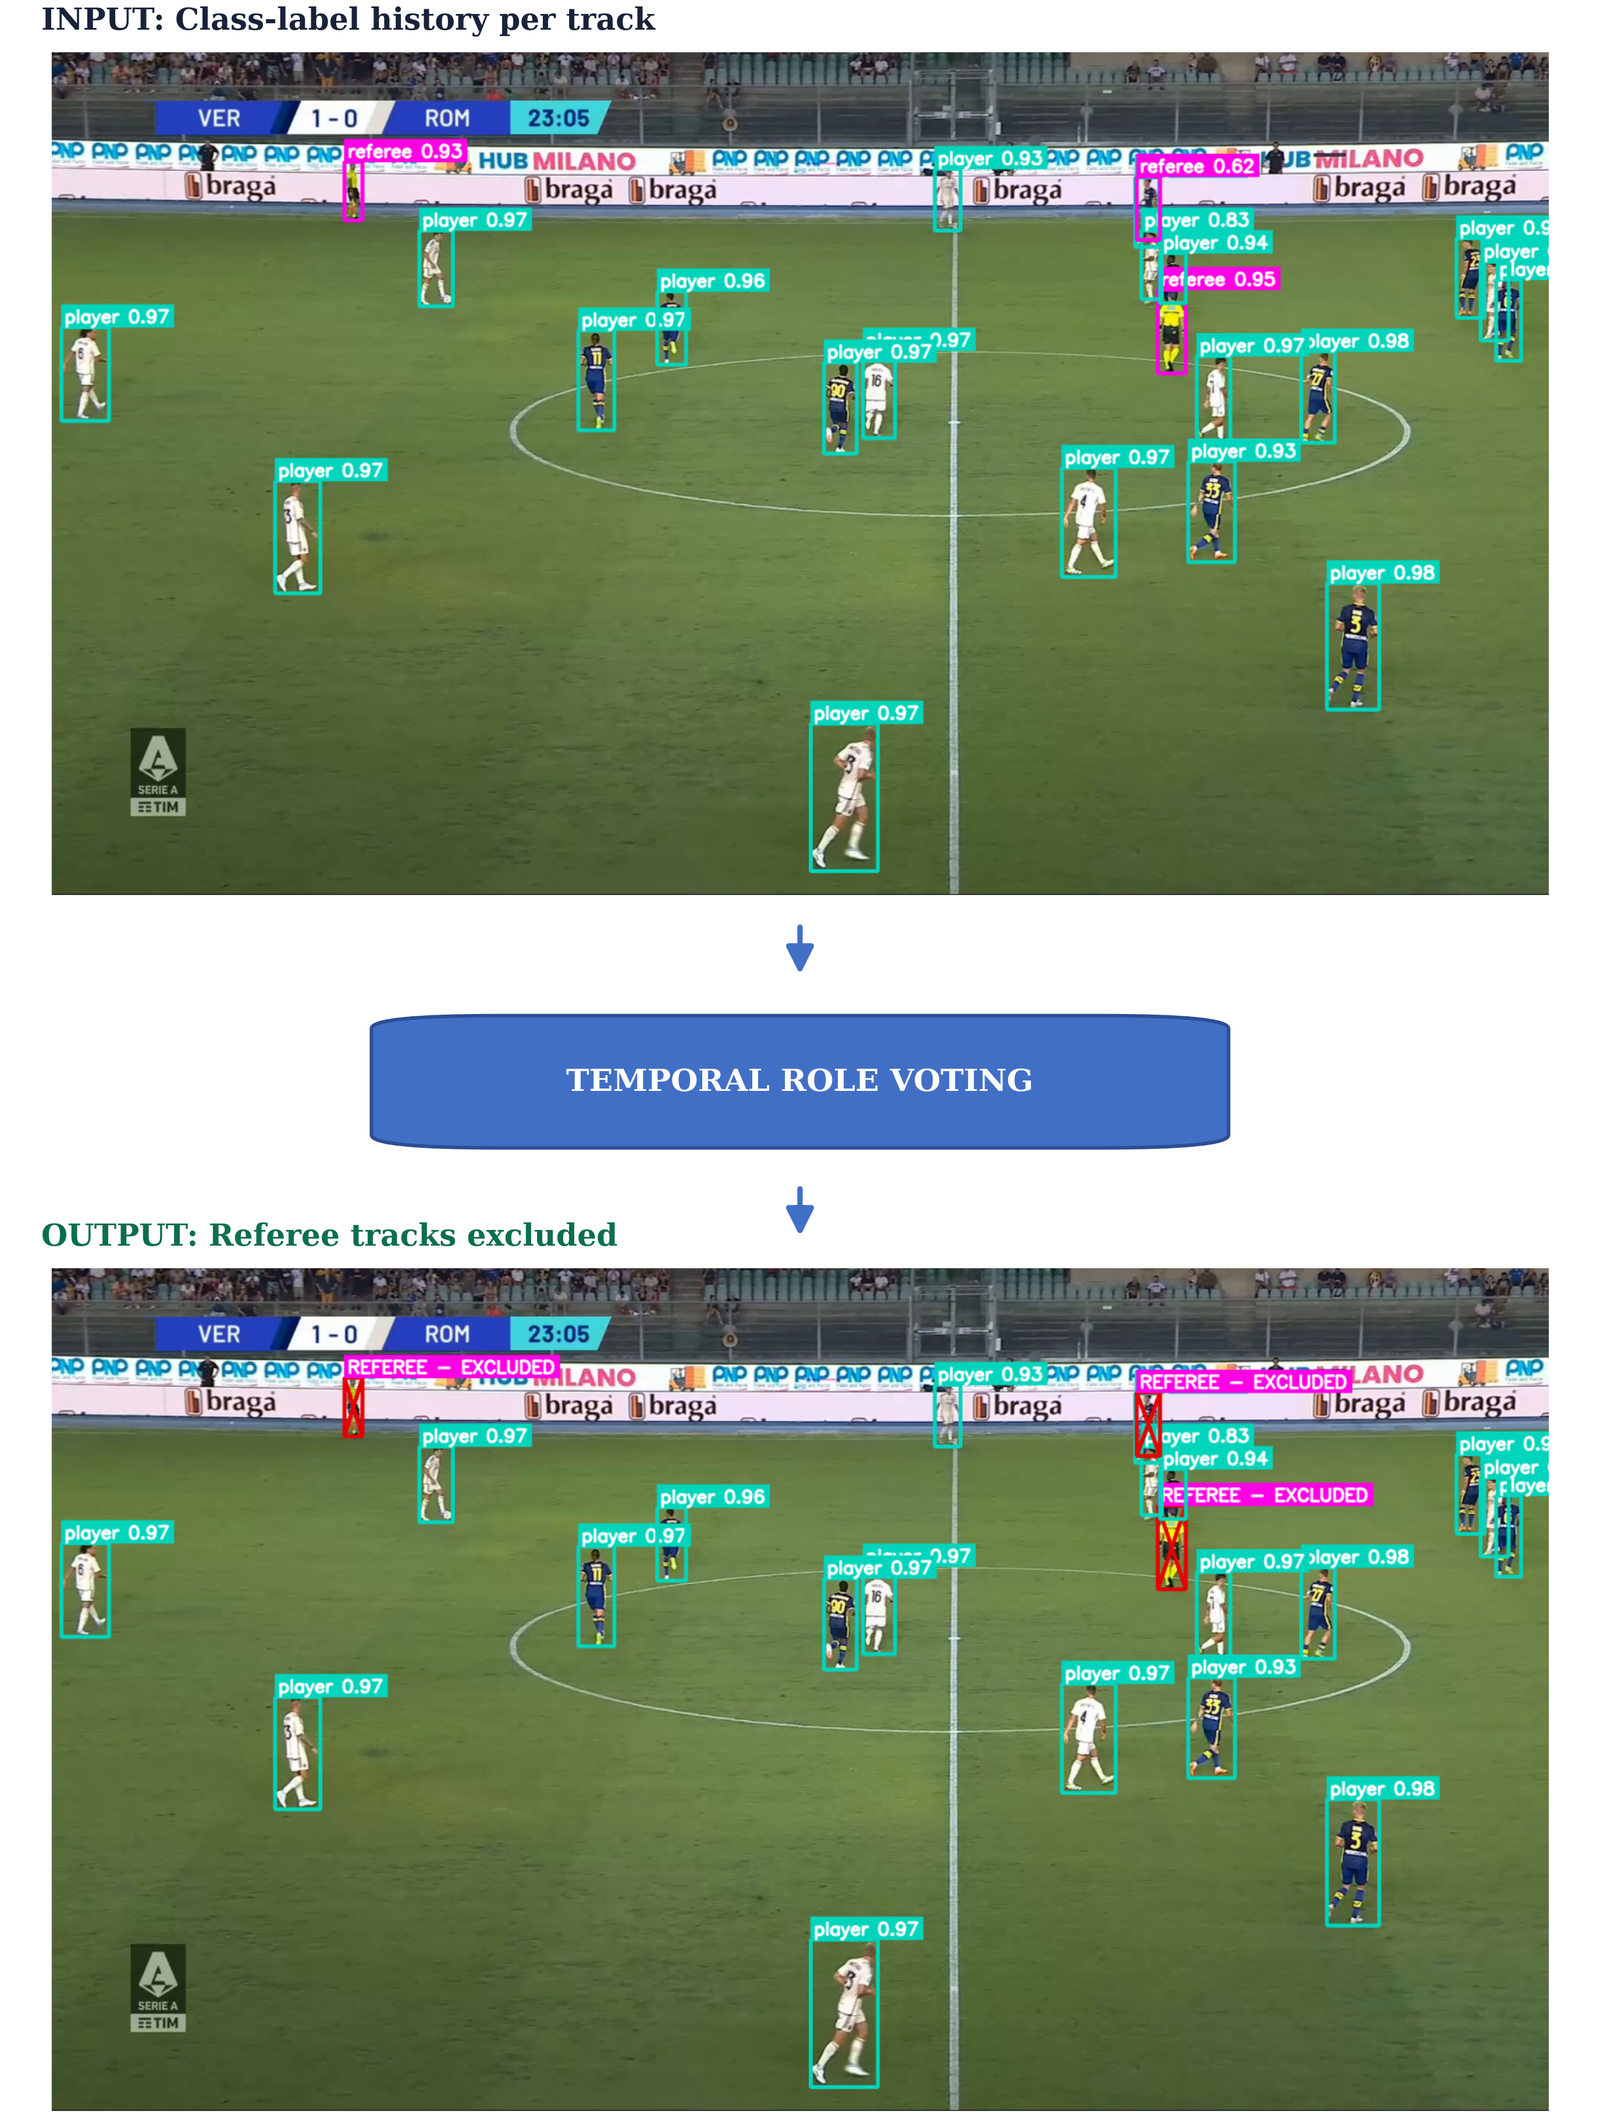
\includegraphics[width=1\textwidth]{figures/steps_video/step_3_figure.png}
    \caption{Temporal role voting (Section~\ref{sec:temporal-voting}).
    Using the class-label history accumulated for each track, the
    \texttt{TemporalRoleVoter} locks tracks whose observed class is
    predominantly \textit{referee} and excludes them from further OCR
    processing, as shown by the ``REFEREE --- EXCLUDED'' annotation.}
    \label{fig:video-step3-role}
\end{figure}

\begin{figure}[H]
    \centering
    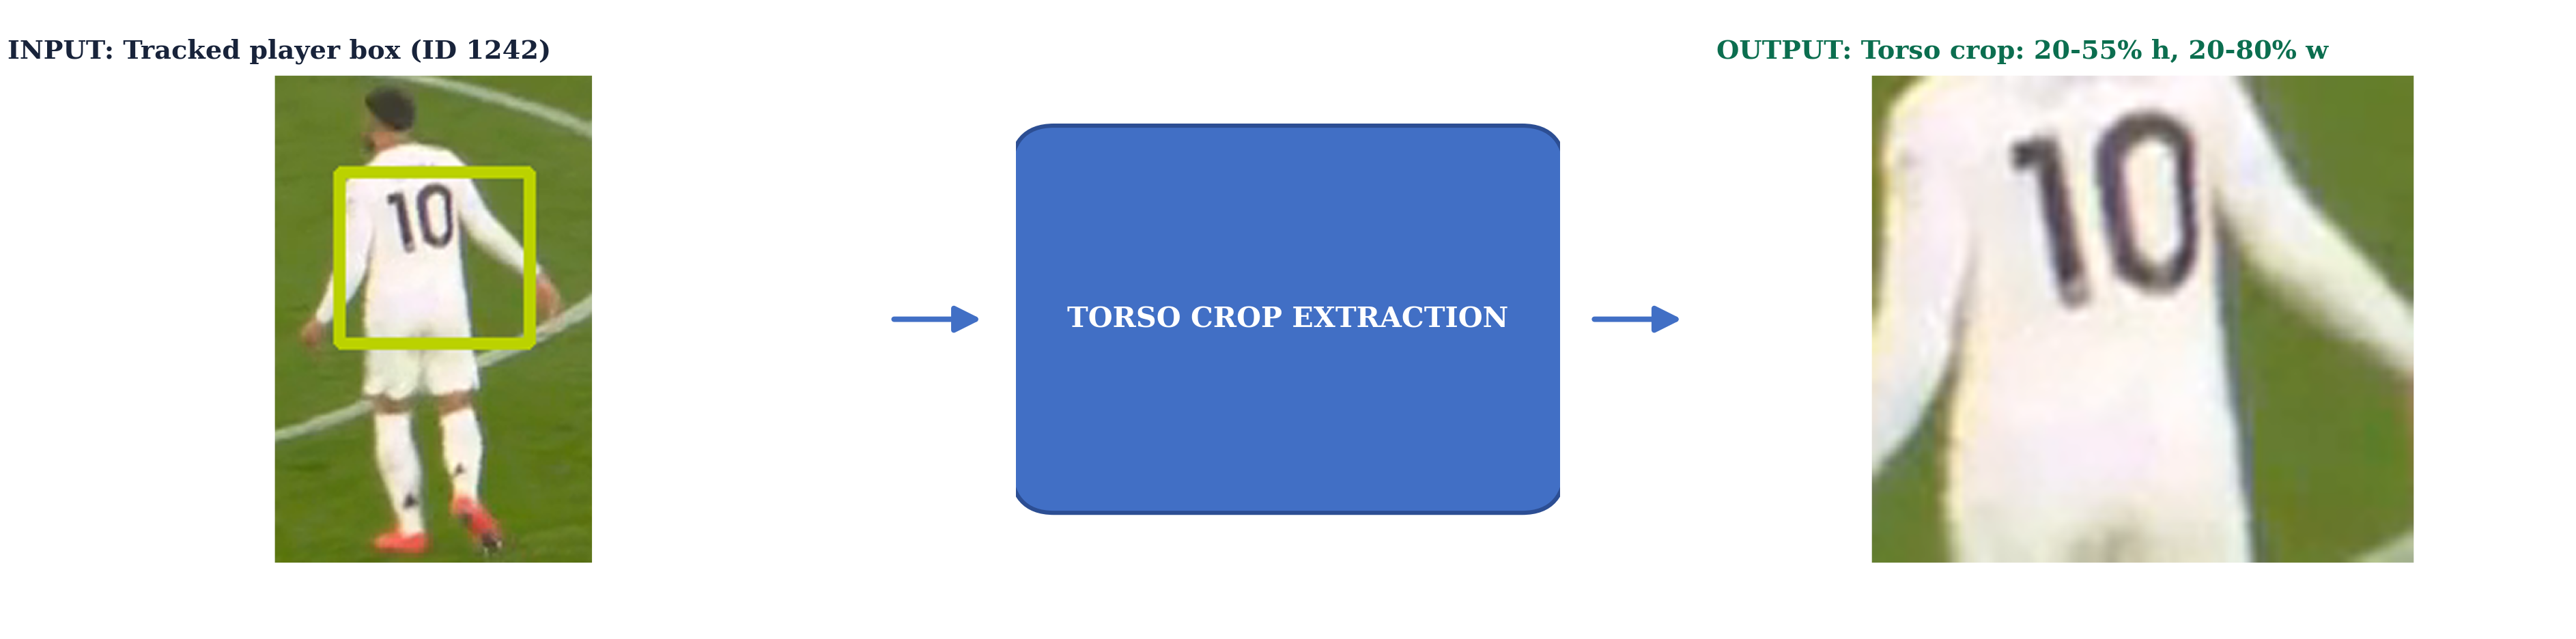
\includegraphics[width=1\textwidth]{figures/steps_video/step_4_figure.png}
    \caption{Torso crop extraction. For non-referee track 1242, the
    torso region spanning 20--55\% of box height and 20--80\% of box
    width is extracted from the tracked player box, following the
    fixed-fraction heuristic described in
    Section~\ref{sec:models}.}
    \label{fig:video-step4-torso}
\end{figure}

\begin{figure}[H]
    \centering
    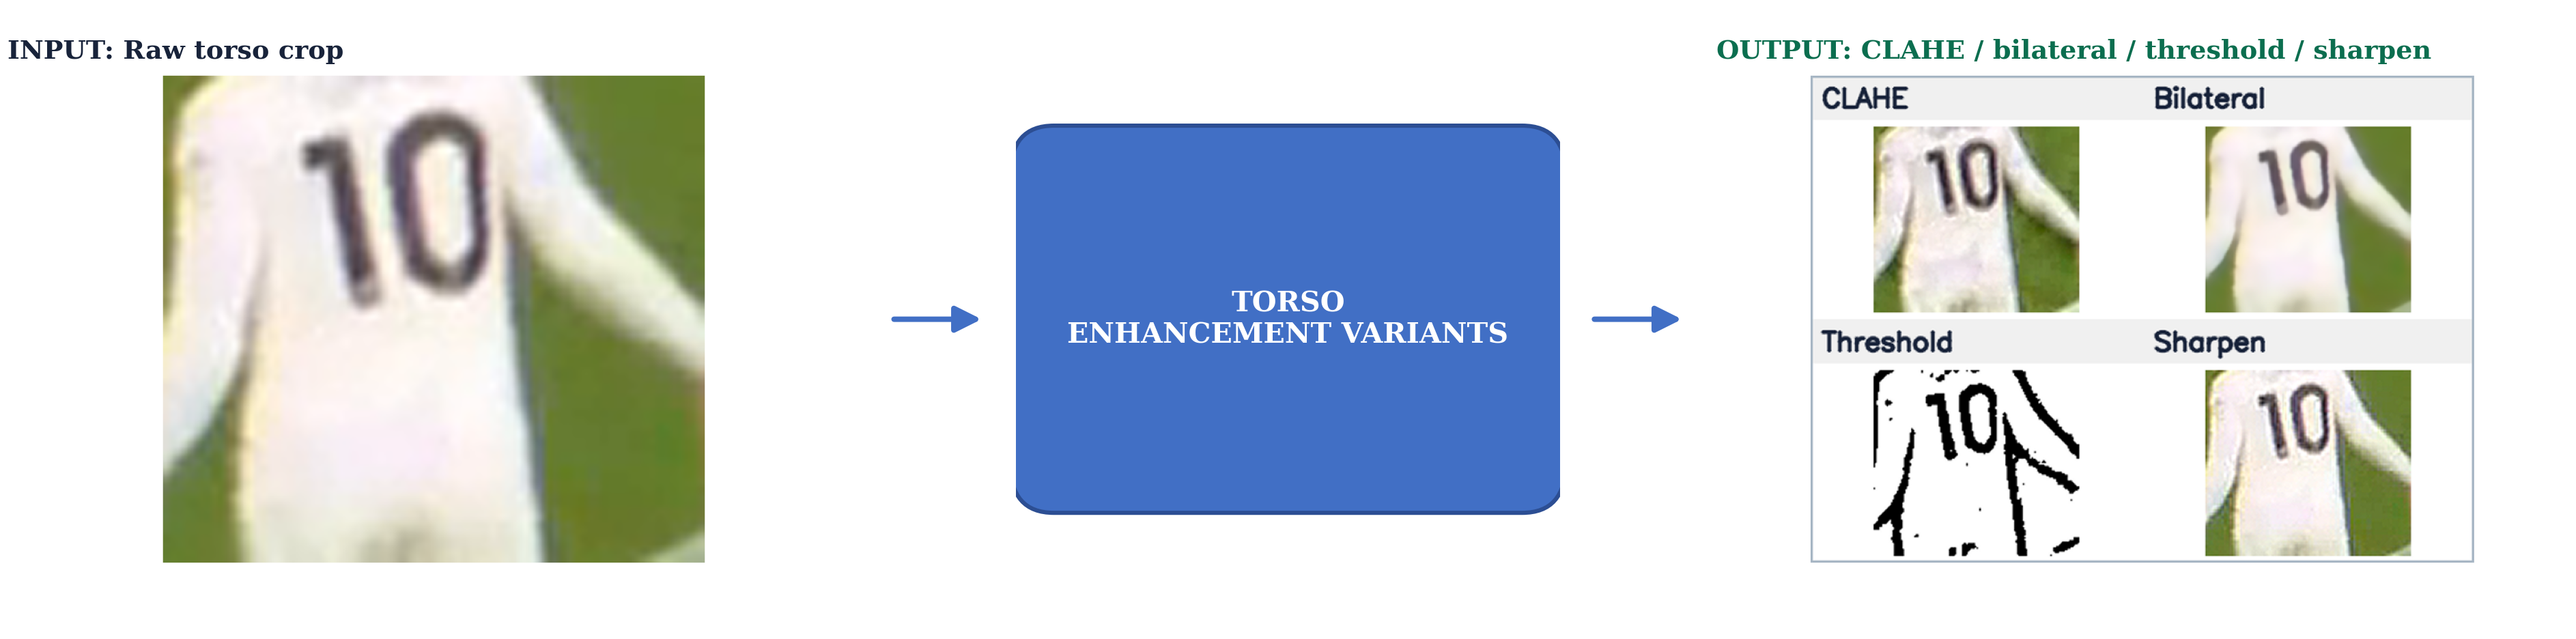
\includegraphics[width=1\textwidth]{figures/steps_video/step_5_figure.png}
    \caption{Torso crop enhancement (Section~\ref{sec:preprocessing}).
    The raw torso crop is processed into four enhancement variants ---
    CLAHE, bilateral-filter-plus-CLAHE, adaptive threshold, and
    high-pass sharpening --- each independently offered to the OCR
    stage.}
    \label{fig:video-step5-enhance}
\end{figure}

\begin{figure}[H]
    \centering
    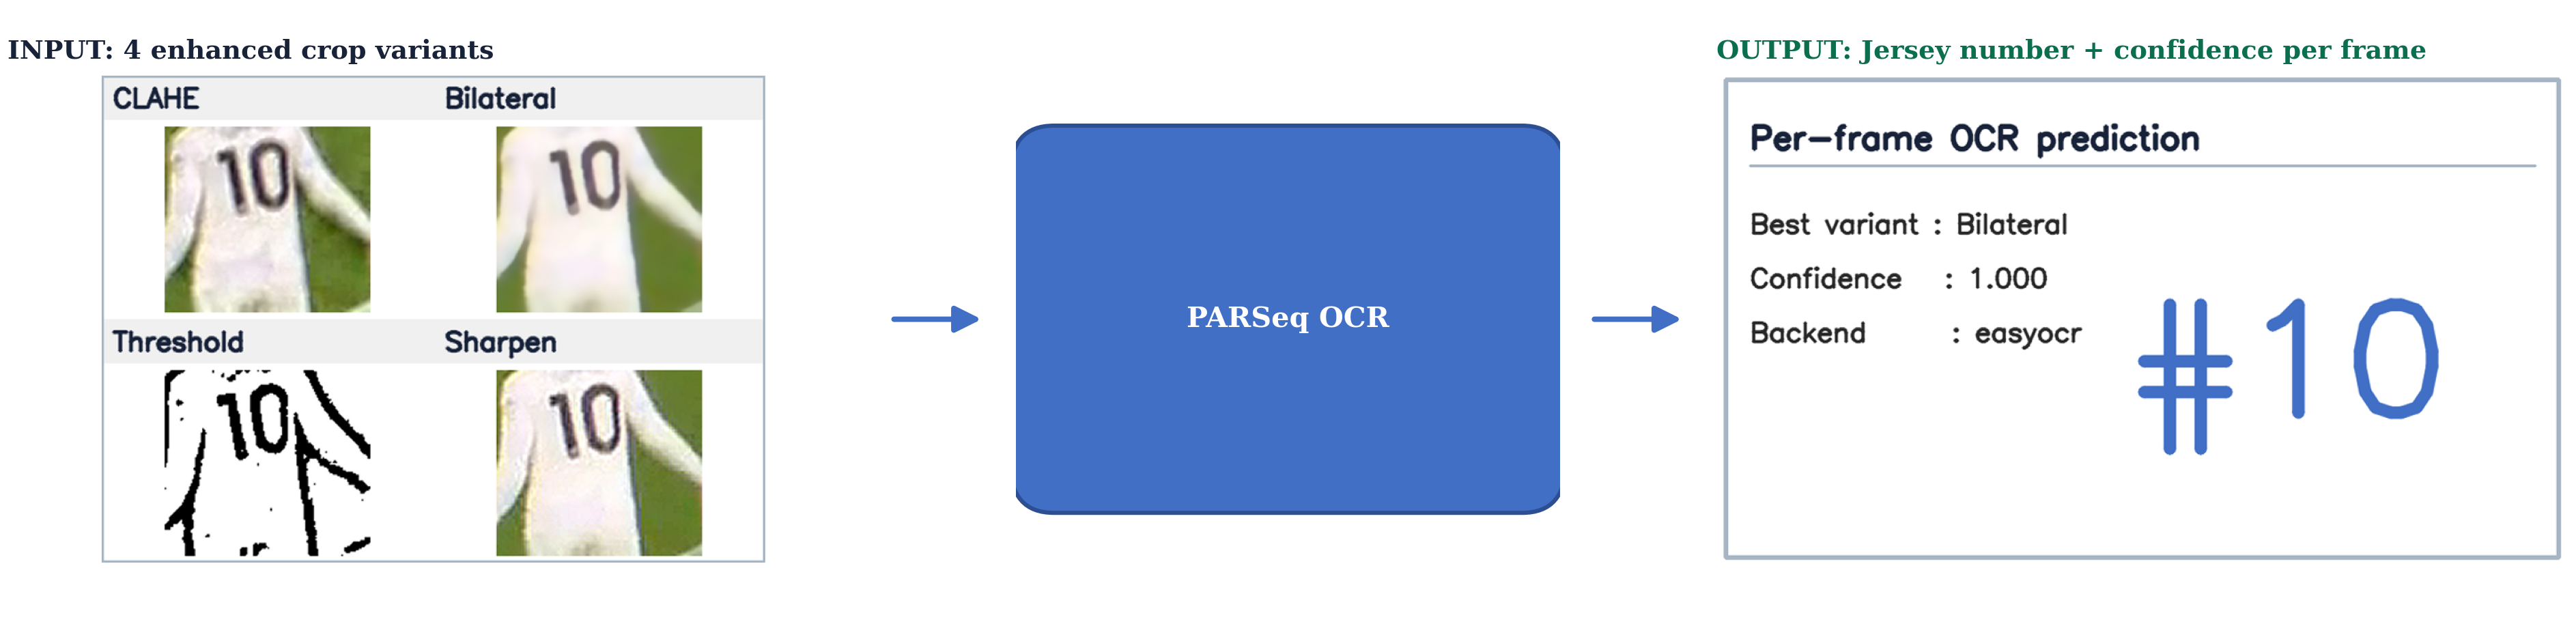
\includegraphics[width=1\textwidth]{figures/steps_video/step_6_figure.png}
    \caption{Jersey OCR on the four enhanced variants. The best-scoring
    variant and its confidence are reported together with the
    \emph{active backend}; in this particular frame the pipeline had
    fallen back to EasyOCR, providing a concrete illustration of the
    PARSeq-with-EasyOCR-fallback design described in
    Section~\ref{sec:models}.}
    \label{fig:video-step6-ocr}
\end{figure}

\begin{figure}[H]
    \centering
    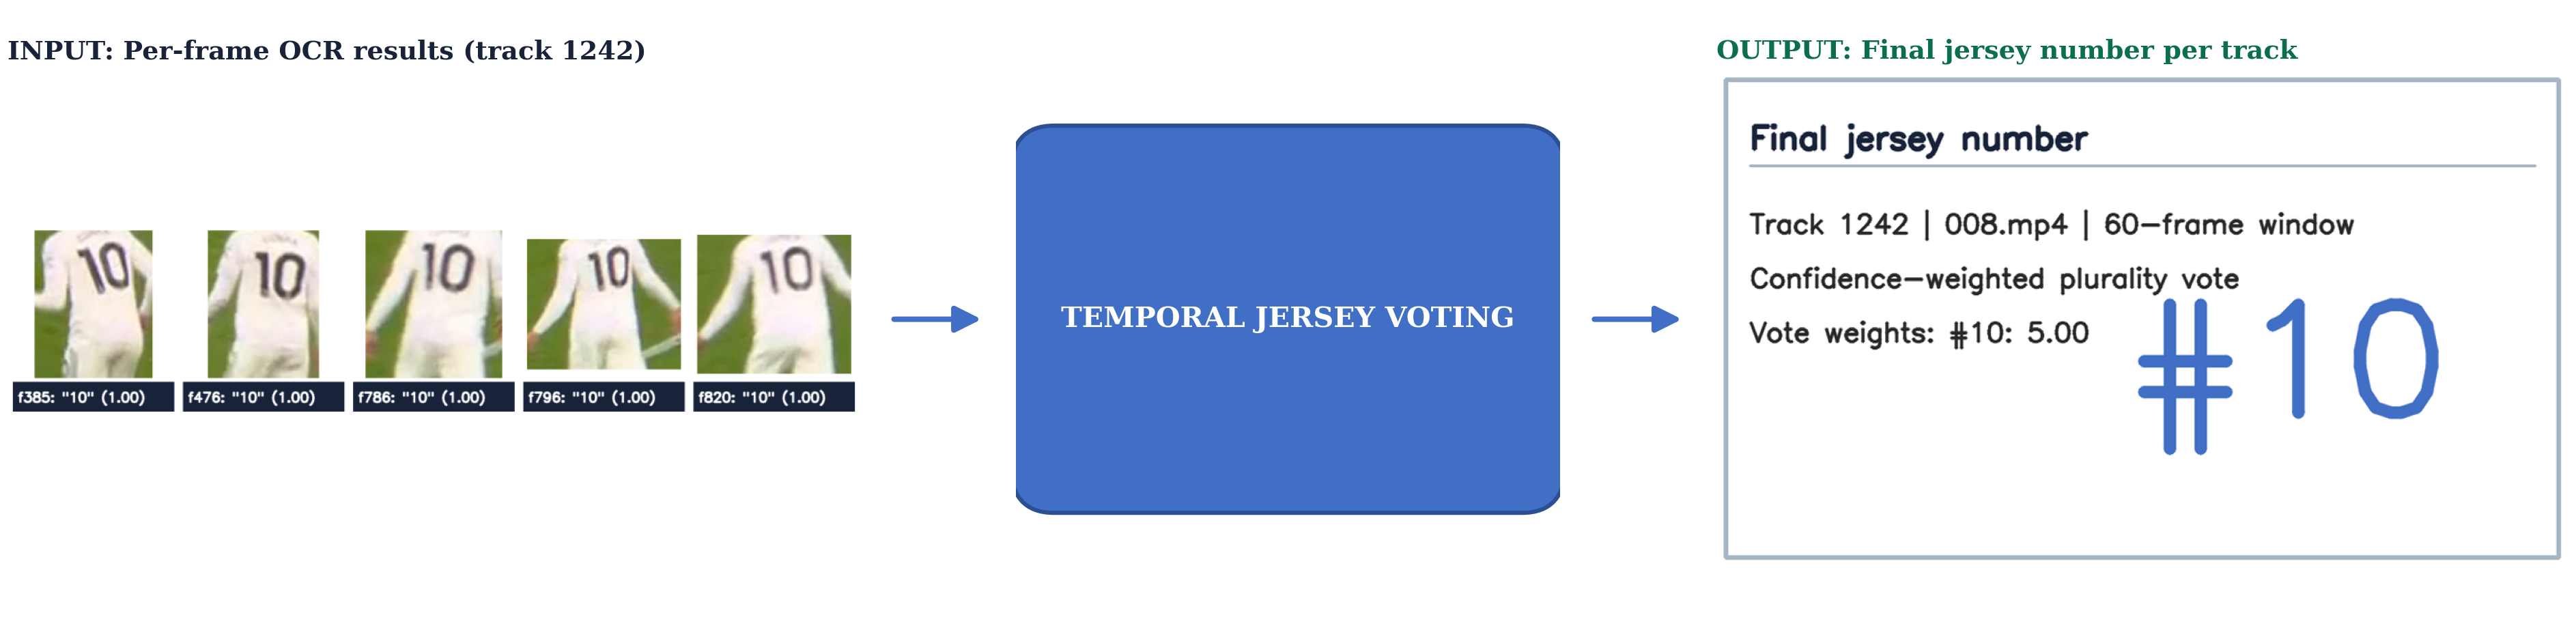
\includegraphics[width=1\textwidth]{figures/steps_video/step_7_figure.png}
    \caption{Temporal jersey voting (Equation~\ref{eq:temporal-vote}).
    Per-frame OCR observations for track 1242 within the 60-frame
    window (e.g.\ frames 385, 476, 786, 796, 820, each reading ``10''
    with confidence 1.00) accumulate confidence-weighted support for
    each candidate number, and the highest-weighted candidate is
    reported as the track's final jersey number.}
    \label{fig:video-step7-voting}
\end{figure}

\begin{figure}[H]
    \centering
    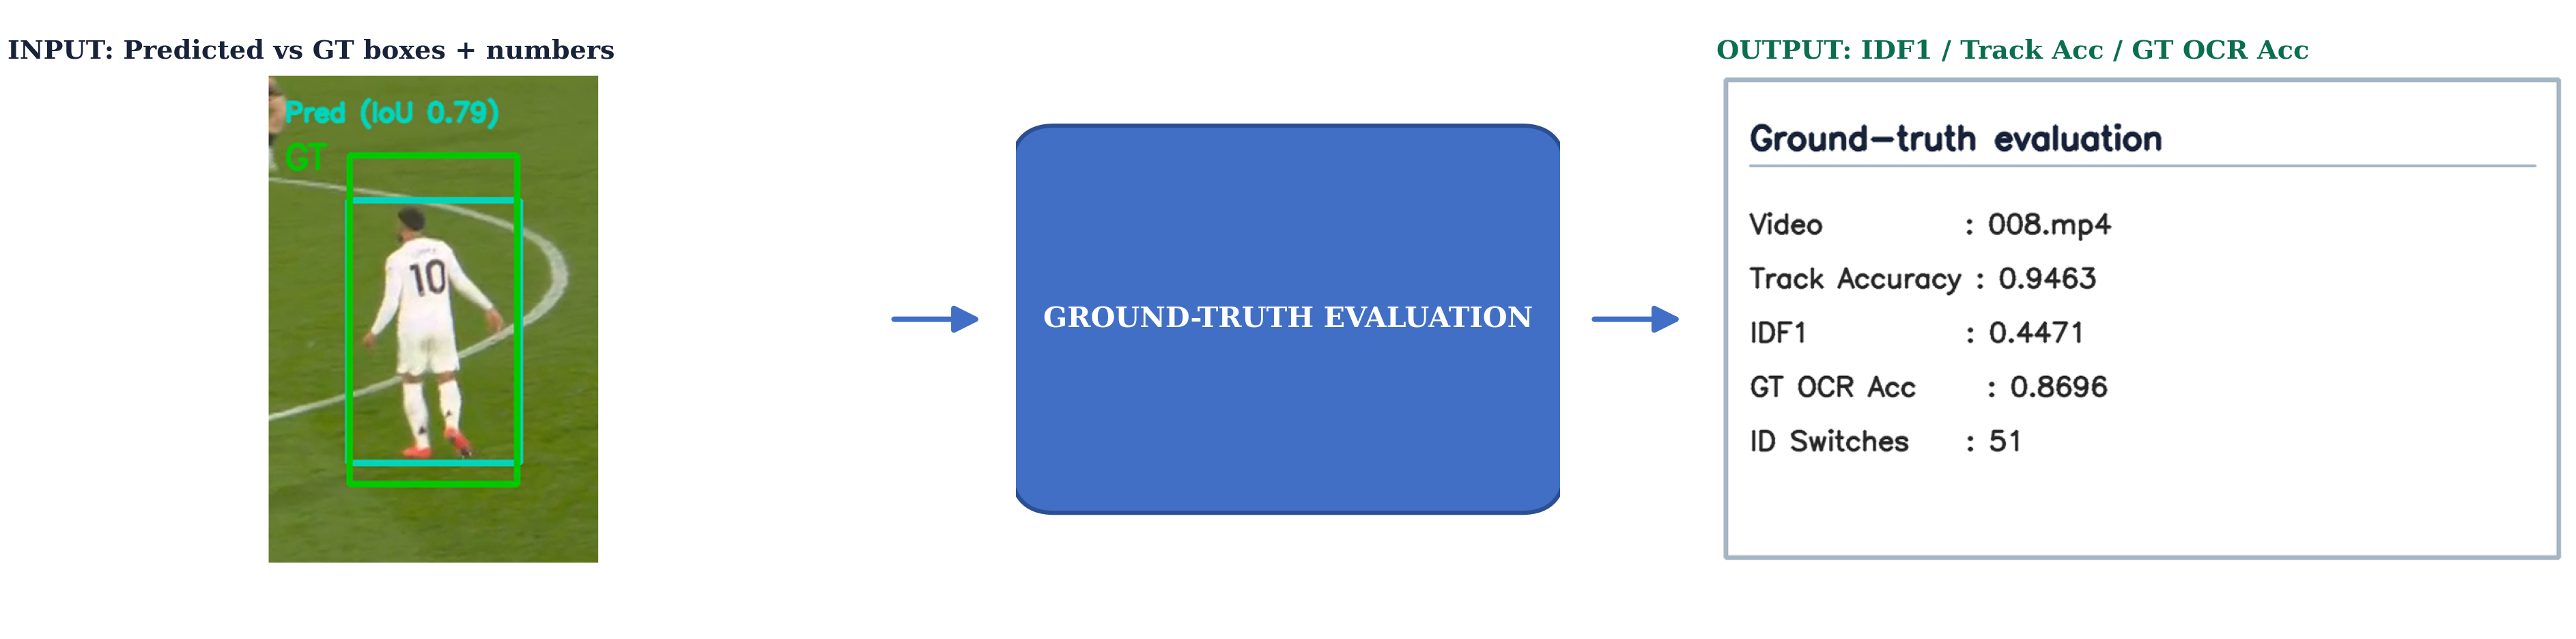
\includegraphics[width=1\textwidth]{figures/steps_video/step_8_figure.png}
    \caption{Ground-truth evaluation (Section~\ref{sec:gt-eval}). The
    predicted track and jersey number are matched against manually
    annotated ground-truth boxes and numbers for the same clip
    (008.mp4), yielding the per-video tracking accuracy, IDF1, and GT
    OCR accuracy metrics reported in Chapter~\ref{ch:results}.}
    \label{fig:video-step8-gteval}
\end{figure}
